\documentclass{article}
\usepackage{iclr2027_conference,times}
\usepackage{amsmath,amssymb,graphicx,booktabs,hyperref,url}
\usepackage{array}
\usepackage{wrapfig}
\usepackage{float}
% Balance body spacing across nine pages; retain template dimensions and fonts.
\linespread{1.015}
\setlength{\parskip}{0pt}
\setlength{\parindent}{1em}
\setlength{\abovedisplayskip}{5pt plus 2pt minus 2pt}
\setlength{\belowdisplayskip}{5pt plus 2pt minus 2pt}
\setlength{\abovedisplayshortskip}{3pt plus 2pt}
\setlength{\belowdisplayshortskip}{3pt plus 2pt}
\setlength{\textfloatsep}{8pt plus 2pt minus 2pt}
\setlength{\floatsep}{6pt plus 2pt minus 2pt}
\setlength{\intextsep}{6pt plus 2pt minus 2pt}
\setlength{\abovecaptionskip}{3pt}
\setlength{\belowcaptionskip}{2pt}
\raggedbottom
% Preserve ICLR heading styles without adding a titlesec dependency.
\makeatletter
\renewcommand{\section}{\@startsection{section}{1}{\z@}
  {-8pt plus -2pt minus -1pt}{4pt}{\large\sc\raggedright}}
\renewcommand{\subsection}{\@startsection{subsection}{2}{\z@}
  {-6pt plus -2pt minus -1pt}{3pt}{\normalsize\sc\raggedright}}
\renewcommand{\subsubsection}{\@startsection{subsubsection}{3}{\z@}
  {-5pt plus -1pt minus -1pt}{2pt}{\normalsize\sc\raggedright}}
\renewcommand{\paragraph}{\@startsection{paragraph}{4}{\z@}
  {4pt plus 1pt minus 1pt}{-1em}{\normalsize\bf}}
\makeatother
\renewcommand{\topfraction}{0.92}
\renewcommand{\bottomfraction}{0.85}
\renewcommand{\textfraction}{0.07}
\renewcommand{\floatpagefraction}{0.75}
\newcommand{\tabdir}{tables}
\makeatletter
\newcommand{\tableinput}[1]{\@@input \tabdir/#1 }
\makeatother
\title{Chip Capacitance Prediction by a Jointly Routed Transformer}
\author{Anonymous authors}
\begin{document}
\maketitle


\begingroup
\renewcommand\thefootnote{}
\footnotetext{
Anonymous code and reproducibility artifacts are available at

\url{https://anonymous.4open.science/r/residual-gating-capacitance-9727/}
}
\addtocounter{footnote}{-1}
\endgroup

\begin{abstract}
Accurate parasitic capacitance estimation is essential for chip design and verification.
Lookup-table-based parasitic extraction (LUT-based PEX) reuses precomputed capacitance tables to avoid weeks to months of physical simulations, but sparse coverage limits accuracy for unobserved chip layout geometries.
To address this limitation, we propose a jointly routed Transformer for chip capacitance prediction, conditioned on layout geometry, material context, and available capacitance observations.
Our key idea is to train a shared Transformer to jointly learn residual corrections to an interpolation estimate and adaptive weights for combining neural and numerical corrections.
Notably, the model extrapolates beyond the observed geometry range and enables transfer to an unseen manufacturing process without parameter updates, aided by our structured tokenizer.
Moreover, we curate and augment a unified dataset and evaluation suite for capacitance prediction from sparse observations, advancing AI research in LUT-based PEX.
Our method outperforms commercial-style multilinear interpolation in all 15 evaluated settings and reduces normalized extrapolation error by 84--86\% on public tables.
Encouragingly, these gains extend to downstream chip analysis: timing estimates using our predicted capacitances more closely match the full-table reference in all 16 settings across eight fixed layouts.
\end{abstract}

\section{Introduction}
\label{sec:introduction}

Accurate parasitic capacitance estimation is essential for chip design and
verification because capacitance affects signal delay and coupling between
wires~\citep{yu2021pex}.
Parasitic extraction (PEX) supplies these estimates for static timing analysis
(STA) and circuit simulation. Field solvers compute capacitance from
electrostatics~\citep{nabors1991fastcap}, but characterizing many geometries is
expensive. Lookup-table-based PEX (LUT-based PEX) reuses precomputed values through lookup and
interpolation~\citep{openrcx}, as illustrated in Figure~\ref{fig:pex_overview}.
Sparse tables reduce characterization costs but limit prediction accuracy
within and beyond the observed geometry range, motivating better interpolation
and extrapolation from available observations.

\begin{figure}[t]
\centering
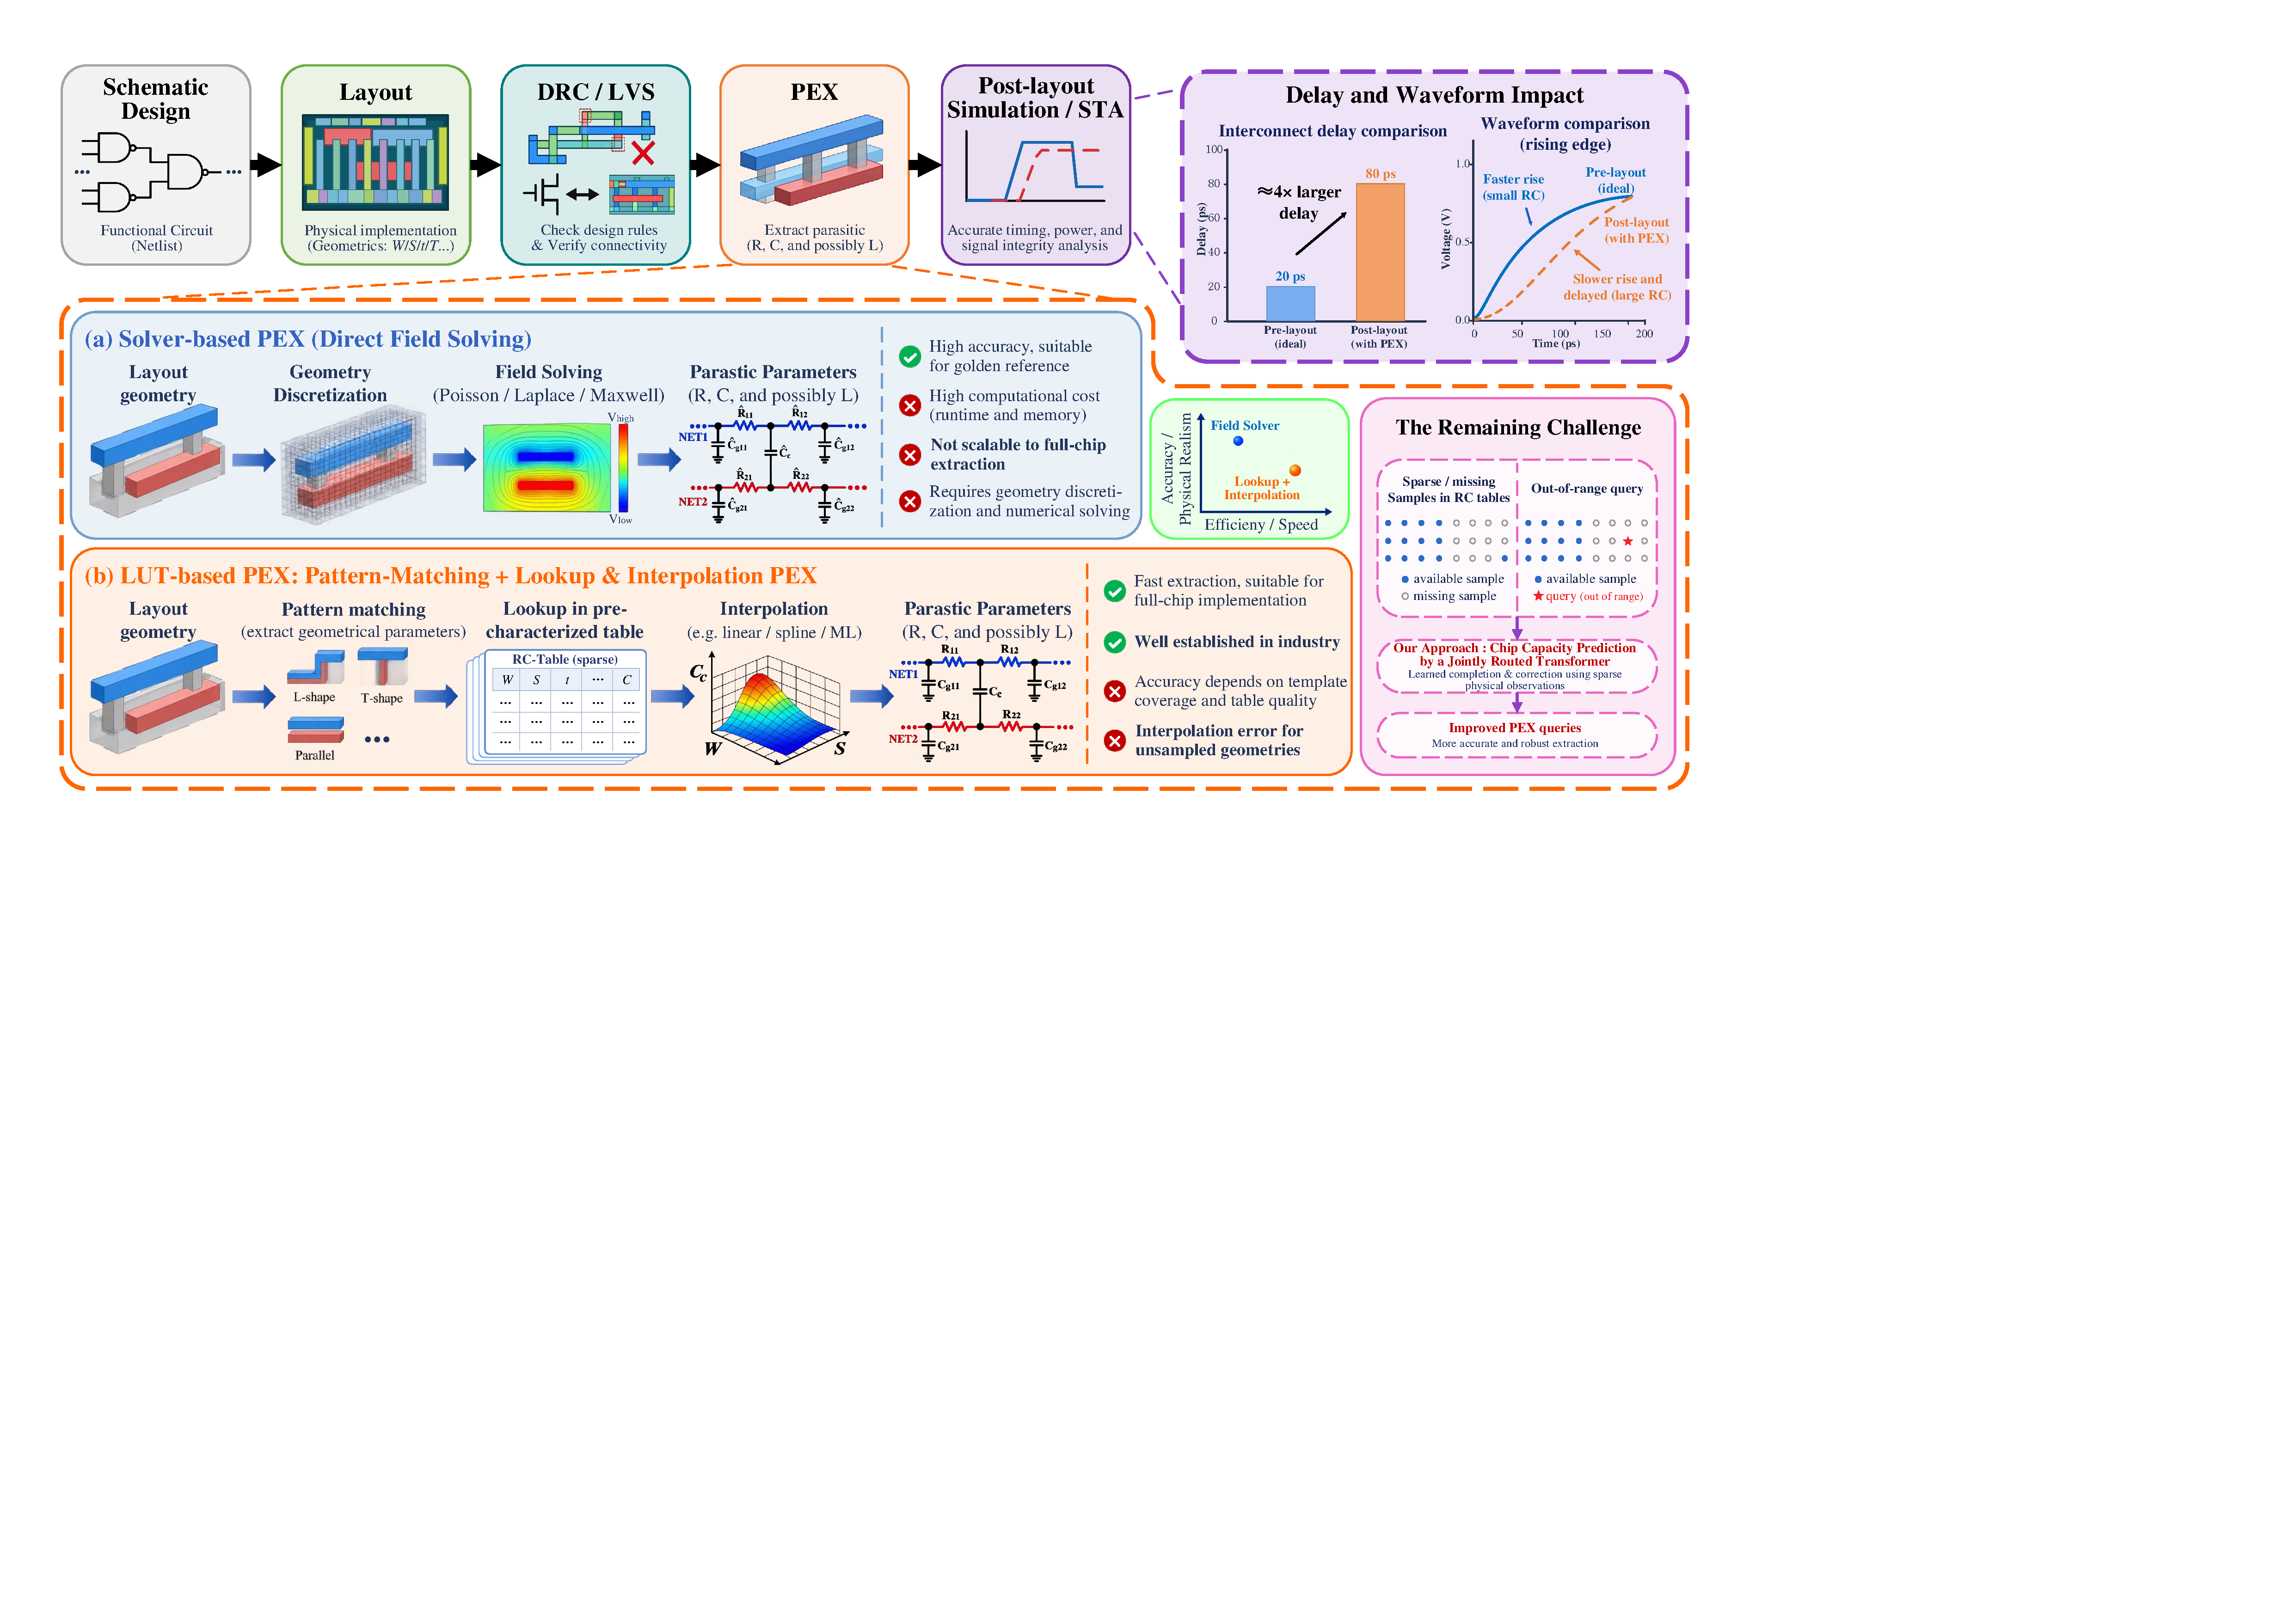
\includegraphics[width=\linewidth]{figure/pex_prediction_overview.pdf}
\caption{Parasitic extraction by (a) field solving or (b) characterized patterns.
We predict capacitance from sparse observations and audit its downstream timing effects.}
\label{fig:pex_overview}
\end{figure}

Existing learning-based methods predict capacitance from geometry using
multilayer perceptrons~\citep{kasai2019nn}, convolutional and graph
networks~\citep{cnncap,liu2024gnncap}, and point-cloud and attention-based
Transformers~\citep{guo2024pctcap,attentioncap}.
Residual and hybrid approaches combine learned models with physical or numerical
methods~\citep{tsai2025rescap,abouelyazid2022hybrid}.
However, direct surrogates encode physical responses in model parameters,
making generalization sensitive to training coverage. Recent work on interconnect
geometry exploration reports rising errors near training thickness boundaries,
requiring broader coverage to maintain accuracy~\citep{tsai25}.
Rule tables already contain valuable process-specific physical calculations.
We therefore provide observed geometry--capacitance pairs at inference,
conditioning queries on the current table's sparse observations and material
context, following the principle of learning from context
sets~\citep{garnelo2018cNP,kim2019anp}.
Here, extrapolation is relative to the current observations, rather than
necessarily to the source training distribution.
Appendix~\ref{app:related-work} discusses related work in detail.

We propose a jointly routed Transformer for chip capacitance prediction.
Our key idea is to jointly learn residual corrections to an interpolation
estimate and adaptive weights for combining neural and numerical corrections.
A structured tokenizer encodes geometry, material context, and available
capacitance observations, allowing a shared Transformer to condition both
prediction and input-dependent routing~\citep{rosenbaum2018routing} on each table.
The neural residual allows predictions beyond clamped interpolation boundaries.
Notably, observation conditioning supports transfer to an unseen manufacturing
process without parameter updates.

Motivated by public benchmarks for AI in chip design~\citep{circuitnet2},
we curate a unified LUT-based PEX dataset and evaluation suite combining rule
tables from four manufacturing technologies, an independent finite-element
reference, and a source-only transfer protocol. Controlled observation masks
enable separate evaluation of interpolation and extrapolation.
At 30\% missingness, our method outperforms rank-matched commercial-style
multilinear interpolation in all 15 evaluated settings and reduces normalized
extrapolation error by 84--86\% on public tables.
Encouragingly, incorporating predictions into extraction rules improves
agreement with full-table capacitance and timing estimates in all 16 downstream
settings across eight fixed layouts.
\textbf{Our main contributions are summarized as follows:}
\begin{itemize}
\item \textbf{A generalizable neural framework for LUT-based PEX.}
To our knowledge, we are the first to introduce a neural framework
that enhances LUT-based PEX through both geometry extrapolation
and cross-process transfer without parameter updates.
\item \textbf{A unified dataset and evaluation suite.}
We curate and augment capacitance tables from four manufacturing
technologies with independently solved reference grids, establishing
a unified benchmark for interpolation, extrapolation, and
source-only cross-process transfer.
\item \textbf{Downstream validation.}
Experiments on eight fixed routed layouts demonstrate
improved agreement with full-table capacitance and timing estimates in all
16 evaluated settings.
\end{itemize}

\section{Terminology}
\label{sec:terminology}

\paragraph{Capacitance tables and material stacks.}
A capacitance table maps sampled wire geometries to capacitance components.
Each row corresponds to a geometry $x_i$ and a response vector $y_i$;
$X$ denotes all candidate geometries and $K$ the number of response components.
A material stack describes the conductor and dielectric layers of a process.
The context $c$ encodes structural and material information associated with
these geometries. A table stores sampled values of the capacitance response;
the prediction task estimates responses at supplied, unobserved query geometries.

\paragraph{Support, queries and masks.}
The support $S$ is the set of observed row indices, with available responses
$y_S$. The query set $\mathcal{Q}$ contains the remaining indices whose
responses must be predicted. A mask determines which responses are hidden;
query coordinates remain available. \emph{Support-conditioned} means that a
prediction depends on the current table's observed geometry--response pairs.
The missingness rate is the fraction of candidate rows hidden by the mask.

\paragraph{Support rank and prediction regimes.}
Support rank counts the independent geometric directions spanned by the
observed coordinates, which can be fewer than the number of stored coordinates.
An \emph{in-support} query lies inside the observed support's convex hull in its
affine span; an \emph{out-of-support} query lies outside that supported region.
These terms refer to the current observations, not the support of a training
distribution or the extent of the original reference table. Random, contiguous-block
and boundary-extrapolation masks specify how observations are withheld.

\paragraph{Anchor, residual and gate.}
The anchor $b_i$ is a deterministic interpolation estimate computed from
observed support. A residual $\Delta_{i,e}$ is a correction relative to this
anchor, supplied by a neural or numerical branch $e$. The gate assigns
nonnegative weights $\pi_{i,e,k}$ that sum to one across applicable branches
for each query $i$ and capacitance component $k$. An \emph{anchor-only}
control returns $b_i$; the full model adds the gated residual corrections.

\paragraph{Source-only transfer.}
The source stack supplies the training data, and the target stack supplies the
tables evaluated after training. Source-only transfer keeps model parameters
fixed while using the target table's available observations as support;
it does not perform target-domain parameter updates.

\section{Method}
\label{sec:method}

\subsection{Task and overall architecture}

We formulate capacitance estimation from sparse observations as conditional
query prediction. Each episode supplies support and query geometries $X=\{x_i\}_{i=1}^{N}$, with
$x_i\in\mathbb{R}^{d}$ ($d=3$ stored coordinates), a structural/material
context $c$, and $K$ capacitance components ($K\in\{2,3\}$).
Only the support $S\subseteq\{1,\ldots,N\}$ has characterized values $y_S$;
the model predicts responses at the query indices
$\mathcal{Q}=\{1,\ldots,N\}\setminus S$. Queries may lie inside or outside
the observed hull. In the experiments, masks partition characterized tables
into support and queries so that withheld responses provide evaluation targets.
Thus, the learned mapping is
$F_\theta:(X,c,S,y_S)\mapsto\hat y_{\mathcal{Q}}$.
All candidate coordinates are known, but query labels are absent from every
input and support computation. Training-derived coordinate scales $\xi$ and
family-specific component scales $\sigma$ are fixed before evaluation.

Figure~\ref{fig:network} summarizes the architecture: a structured tokenizer and
shared Transformer feed a residual head and a component-wise gate. Both heads
use the same query representation, so learning the correction and deciding how
much to trust it are coupled. In physical units,
\begin{equation}
\label{eq:main}
\hat y_{i,k}=\left[b_{i,k}+
 \sum_{e\in\mathcal{E}_i}\pi_{i,e,k}\Delta_{i,e,k}\right]_+,
\qquad \sum_{e\in\mathcal{E}_i}\pi_{i,e,k}=1,
\qquad \pi_{i,e,k}\geq0,
\end{equation}
where $[z]_+=\max(0,z)$, $b_i$ is an observation-derived anchor,
$\Delta_{i,e}$ is a correction to that anchor, and $\mathcal{E}_i$ contains
applicable branches. The network learns \emph{what correction is needed} and
\emph{how strongly to use it} through the same query-prediction objective. We use the term residual gating
for this anchor-centered soft mixture within the routing architecture.

Our design follows three observations about sparse characterization.
First, the table's own support provides a useful numerical reference, so we
learn departures from that reference. Second, local interpolation and learned
extrapolation fail differently as support changes, motivating complementary
correction branches. Third, support quality varies by query and capacitance
component, motivating local routing instead of one fixed mixture per table.

\begin{figure}[t]
\centering
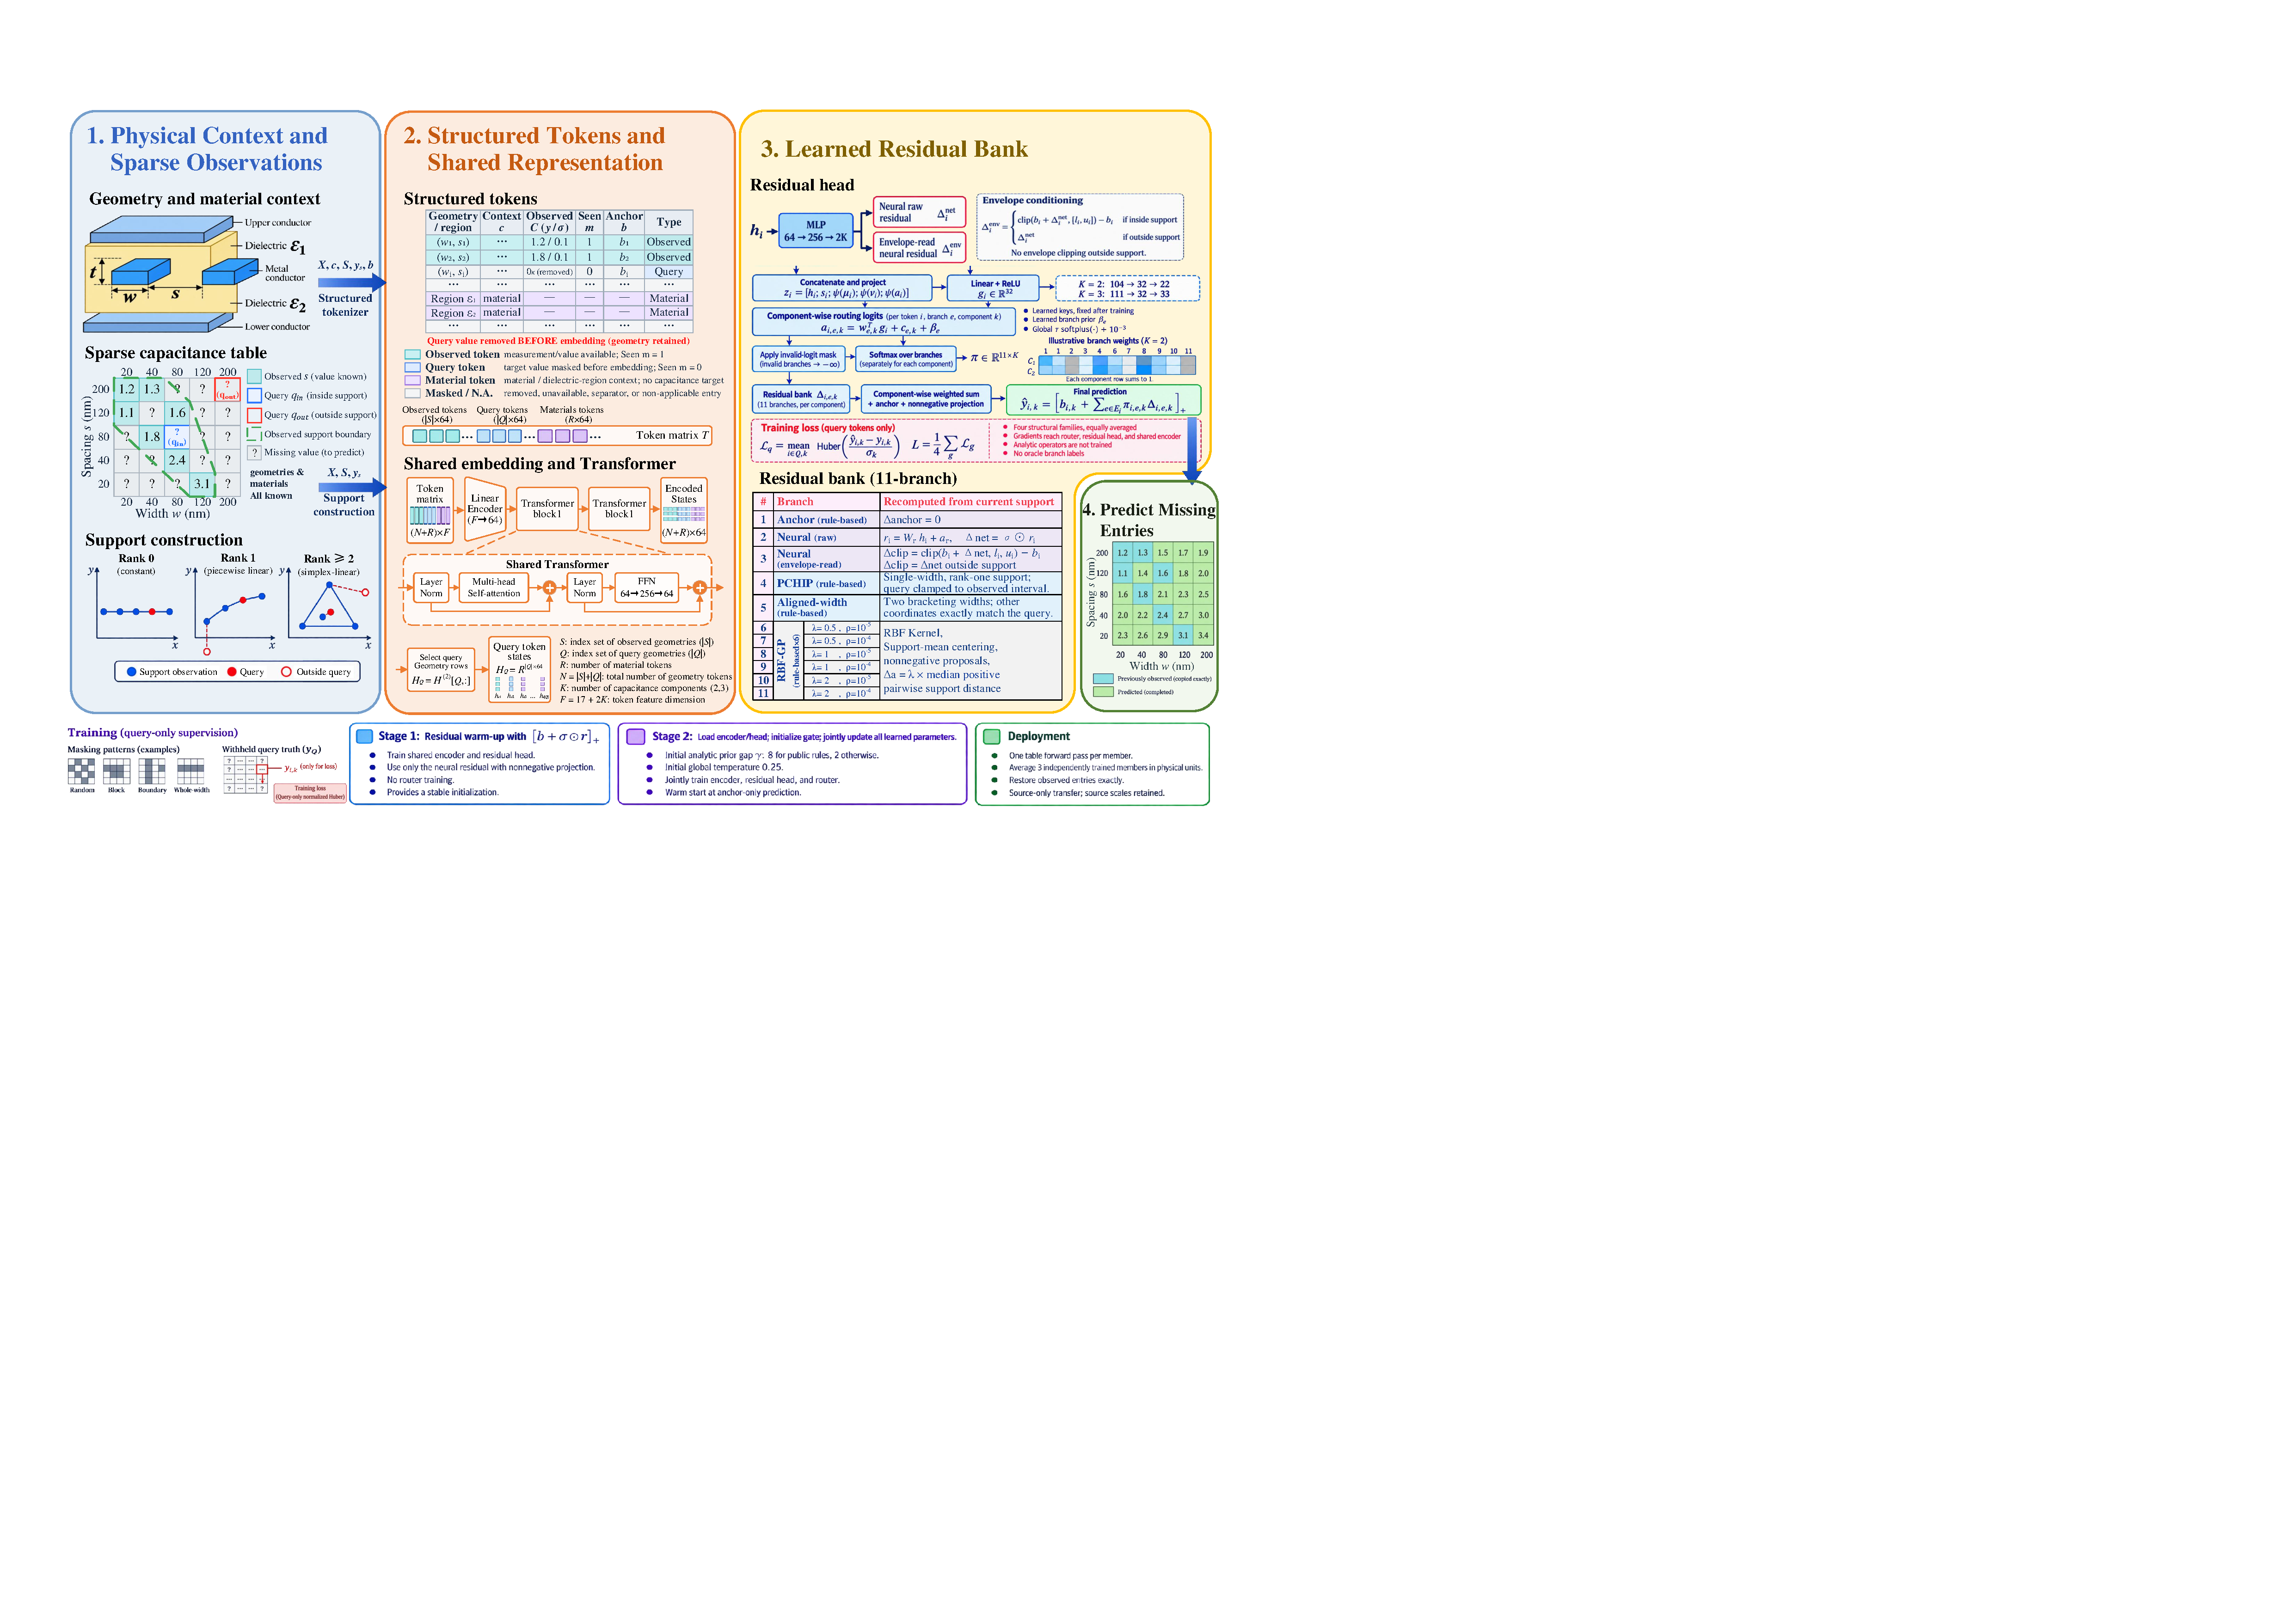
\includegraphics[width=\textwidth]{figure/PEX-fig2.pdf}
\caption{Support-conditioned neural--numerical routing.
Blue: learned modules; gold: numerical computations; green: prediction assembly.
One Transformer supplies the residual and routing state; observed values are preserved.}
\label{fig:network}
\end{figure}

\subsection{Structured geometry--observation tokenization}
\label{sec:tokens}

The tokenizer assigns one numerical token to each candidate geometry and one
to each available dielectric region. Keeping geometry, observation status and
capacitance in the same token preserves their physical correspondence.

\paragraph{Geometry tokens and label removal.}
Let $m_i=\mathbf{1}[i\in S]$. Define
$\tilde y_i=y_i/\sigma$ for $i\in S$ and $\tilde y_i=0$ otherwise;
the zero is an input placeholder, distinguished from a measured zero by $m_i$.
The geometry token is
\begin{equation}
\label{eq:token}
t_i^{\rm geo}=\left[
 \log(1+x_i/\xi)\,;\,c\,;\,\tilde y_i\,;\,m_i\,;\,
 b_i/\sigma\,;\,(1,0)\right]\in\mathbb{R}^{17+2K}.
\end{equation}
Here division and logarithms are componentwise. The 11-dimensional context
$c$ comprises a four-way structural-family indicator
(OVER, UNDER, OVERUNDER, DIAGUNDER; see Appendix~\ref{app:structural-families}
for the structures), the target metal and its two context-layer
indices divided by 16, and three material-summary values (target-conductor bottom height, thickness,
and local relative permittivity) with an availability flag. The material block is zero when unavailable. These family indicators
encode interconnect arrangement, rather than a process-identity vocabulary.
The anchor field exposes the current table's numerical reference to the
encoder, so the learned representation can focus on its correction.

\paragraph{Material tokens.}
For a dielectric region with bottom/top coordinates $z_r^-,z_r^+$ and relative
permittivity $\epsilon_r$, the corresponding token is
\begin{equation}
\label{eq:material-token}
t_r^{\rm mat}=\left[
 \log(1+z_r^-/\xi_1),\log(1+z_r^+/\xi_1),\log(1+\epsilon_r)\,;\,
 c\,;\,0_K\,;\,0\,;\,0_K\,;\,(0,1)\right].
\end{equation}
The type flags distinguish geometry from material despite their common input
width. Material tokens make the dielectric profile directly accessible through
attention, while the summary fields provide a compact table-level context.
Tables without region descriptions simply have no material tokens.

\paragraph{Embedding and information boundary.}
Stacking $N$ geometry and $R$ material tokens gives
$T\in\mathbb{R}^{(N+R)\times(17+2K)}$, projected row-wise to width 64.
Query labels are zeroed \emph{before} embedding; the attention mask excludes
only padding. Explicit physical coordinates replace sequence-index positional
embeddings, and predictions are read from the corresponding geometry tokens.
Appendix~\ref{app:network-details} illustrates the token fields.

\subsection{Support-conditioned Transformer encoder}
\label{sec:encoder}

\begin{equation}
\label{eq:encoder}
\begin{aligned}
 U^{(l)}&=H^{(l-1)}+
  \operatorname{MHSA}_l(\operatorname{LN}(H^{(l-1)})),\\
 H^{(l)}&=U^{(l)}+
  \operatorname{FFN}_l(\operatorname{LN}(U^{(l)})),\quad l=1,2.
\end{aligned}
\end{equation}
Let $H^{(0)}=TW_{\rm in}^{\top}+b_{\rm in}$. We use two pre-normalized
Transformer blocks~\cite{attention}, each with four attention heads of width 16
and a $64\rightarrow256\rightarrow64$ feed-forward network, as in
Eq.~\eqref{eq:encoder}.
Bidirectional attention combines local observations, geometric trends and
material context into $h_i=H_i^{(2)}$. Query geometries can interact, but their
labels remain unavailable. With physical coordinates and no index embedding,
the encoder is permutation equivariant at inference. The feed-forward activation
is ReLU and stage-2 dropout is zero; Appendix~\ref{app:network-details} gives
the attention and padding equations.

\subsection{Support anchor and hybrid residual representation}
\label{sec:anchor}

\paragraph{Geometric reference and local envelope.}
The deterministic support module uses only $(X,S,y_S)$ to construct $b_i$,
a local interval $[\ell_i,u_i]$, and an inside-support indicator $I_i$.
Observed coordinates are range-normalized and reduced to independent axes.
For support rank zero, the anchor copies the constant observation; for rank
one, it uses piecewise linear interpolation with endpoint clamping. At higher
rank it uses simplex-linear interpolation in reduced coordinates, with
nearest-observation fallback outside the reduced hull or upon triangulation
failure. Simplex interpolation and a complete-grid multilinear rule agree on
observed nodes but can differ inside a cell; we evaluate the anchor separately
from the commercial baseline. The inside indicator additionally checks the
original affine span. Inside support, $[\ell_i,u_i]$ is the componentwise range
of the bracketing or simplex vertices. Outside support it records the nearest
observation, but is not imposed on the neural extrapolation branch.

\paragraph{Learned residual branches.}
The encoder's pointwise linear head predicts a normalized correction
$r_i=W_rh_i+a_r$. In physical units, the two neural branches are
\begin{equation}
\label{eq:learned-residual}
\Delta_{i,\rm net}=\sigma\odot r_i,\qquad
\Delta_{i,\rm clip}=\begin{cases}
 \operatorname{clip}(b_i+\Delta_{i,\rm net},\ell_i,u_i)-b_i,&I_i=1,\\
 \Delta_{i,\rm net},&I_i=0.
\end{cases}
\end{equation}
These branches share all parameters. They give the router access to both a
flexible learned correction and its locally range-preserving version, without
training two separate networks. Restricting the clipped reading to supported
queries keeps the model's ability to extrapolate. The local envelope is an
inductive bias from observed values, not a general physical bound on capacitance.

\paragraph{Analytic correction operators.}
\label{sec:dictionary}
Eight additional operators provide complementary local and smooth interpolation
biases: one shape-preserving cubic (PCHIP)~\cite{pchip}, one aligned-width
linear rule, and six RBF Gaussian-process predictors~\cite{gpml} with different
fixed kernel scales and ridges. Together with the zero-correction anchor and
the two neural branches, they form $E=11$ slots. Each analytic operator is
recomputed from the current support, and enters as
$\Delta_{i,e}=f_e(x_i;S,y_S)-b_i$.
PCHIP applies to single-width tables. The aligned-width rule interpolates
between two observed widths only when their other coordinates exactly match
the query. Unsupported or nonfinite proposals are masked out.
Appendix~\ref{app:classical} gives the interpolation formulas and boundary
conventions; Appendix~\ref{app:network-details} specifies the branch settings
and tensor dimensions. Figure~\ref{fig:correction-dictionary} illustrates the
correction dictionary.

The operator types are fixed, but their predictions change with the support;
the neural branches also change with $\theta$. Expressing every proposal as a
correction to the same anchor lets the gate compare them on a common scale.



\subsection{Support-aware component routing}
\label{sec:gate}

\paragraph{Routing state.}
The gate receives both the learned state and an explicit description of the
available evidence. Let $s_i\in\mathbb{R}^{23+d+4K}$ concatenate table context
with support density, distances, bracketing extent, support rank and region,
directional coverage, envelope widths, aligned-width availability, and local
variation/slope/curvature estimated from observed values. These features are
\emph{query-label-free}; they intentionally use known support capacitances.

\begin{equation}
\label{eq:routing-state}
 z_i=[h_i;s_i;\psi(\mu_i);\psi(v_i);\psi(a_i)],\qquad
 g_i=\operatorname{ReLU}(W_gz_i+a_g)\in\mathbb{R}^{32}.
\end{equation}
To summarize branch agreement, define $\bar\Delta_{i,e}=\Delta_{i,e}/\sigma$
and compute, componentwise over applicable branches, its mean $\mu_i$,
standard deviation $v_i$ and range $a_i$. With
$\psi(z)=\operatorname{sgn}(z)\log(1+|z|)$, Eq.~\eqref{eq:routing-state}
constructs the routing state.
Agreement statistics include both neural branches, allowing the routing loss
to reach the residual head through this path as well.

\paragraph{Component-wise attention over correction branches.}
For branch $e$ and capacitance component $k$, the output projection defines
the logits and weights in Eq.~\eqref{eq:routing}.

\begin{equation}
\label{eq:routing}
 a_{i,e,k}=w_{e,k}^{\top}g_i+c_{e,k}+\beta_e,\qquad
 \pi_{i,e,k}=\frac{\exp(a_{i,e,k}/\tau)}
 {\sum_{e'\in\mathcal{E}_i}\exp(a_{i,e',k}/\tau)},\quad e\in\mathcal{E}_i.
\end{equation}
Here $g_i$ is a query-dependent state and $w_{e,k}$ is a learned
branch/component key, fixed after training. Unlike token self-attention, this
routing compares correction branches. Aggregate disagreement keeps the gate
compact, but does not identify which individual branch makes an extreme
proposal; Appendix~\ref{app:ablations} examines this limitation.

Inapplicable logits are masked before softmax. A learned global temperature
$\tau=\operatorname{softplus}(t)+10^{-3}$ controls routing sharpness;
$\beta_e$ is a learned branch prior shared across components.
Different components can therefore prefer different corrections at the same
geometry. Because the anchor is the zero-correction branch, allocating mass to
it continuously attenuates the other corrections while retaining the skip path
in Eq.~\eqref{eq:main}. Nonnegative normalized weights make this a convex
mixture of branch values, followed by the nonnegativity projection.

\subsection{Masked-query training and joint optimization}
\label{sec:training}

\paragraph{Training episodes.}
At each update we sample one episode from each of the four structural families,
first choosing a process and then a training table within that process. We
sample random missingness, a contiguous block, or boundary extrapolation,
adding whole-width masks for tables with multiple widths. The missing rate is
sampled from $\{10,30,50,70\}\%$, with a fresh mask seed.
The tokenizer retains all candidate geometries and exposes only $y_S$.
Supervision uses withheld capacitance responses. Changing the mask changes
both the conditioning observations and whether each query requires interpolation
or extrapolation; the objective is continuous query prediction.

\paragraph{Final-output objective.}
Both the residual head and the router are optimized through the assembled
prediction. For an episode,
\begin{equation}
\label{eq:loss}
 L_g=\frac{1}{K|\mathcal{Q}|}\sum_{i\in\mathcal{Q}}\sum_{k=1}^{K}
 \rho\!\left(\frac{\hat y_{i,k}-y_{i,k}}{\sigma_k}\right),\qquad
 \rho(v)=\begin{cases}v^2/2,&|v|\leq1,\\|v|-1/2,&|v|>1.\end{cases}
\end{equation}
The reported stage-2 objective is $L=\tfrac14\sum_gL_g$.
Group-DRO~\cite{dro} is available in the implementation, but its update rate is
zero in this configuration. Huber loss is a robust, normalized training
objective; evaluation separately reports NRMSE. Gradients from Eq.~\eqref{eq:loss}
flow through the mixture weights, the learned corrections and their shared
encoder. Analytic support operators need no learned weights or surrogate risk
labels. Nonnegativity, exact support retention and the optional envelope
reading provide structural constraints; no additional physics penalty is
included in this stage-2 objective.

\paragraph{Residual initialization followed by joint fitting.}
Stage 1 trains the same tokenizer/encoder and a residual prediction head using
$[b+\sigma\odot r]_+$, before introducing the correction bank. Stage 2 loads
that encoder and head, initializes the gate, and updates all network parameters
jointly. The new gate output projection is initially zero; its priors are zero
for the anchor/neural branches and $-\gamma$ for the eight analytic corrections.
We use $\gamma=8$ for public rules and $\gamma=2$ for the other domains, with
$\tau$ initially $0.25$. This suppresses analytic corrections before routing is
learned while retaining gradients to the pretrained residual. A randomly
initialized residual head has zero output, but the warm-started head is already
trained; the full stage-2 model is therefore not claimed to start exactly at
the anchor. AdamW uses learning rate $2\times10^{-4}$, weight decay $10^{-4}$
and unit-norm gradient clipping for 24{,}000 public-domain or 12{,}000
reference/transfer stage-2 updates. Validation ablations support residual
initialization followed by joint optimization; Appendix~\ref{app:ablations}
reports these comparisons, training-budget and branch-prior sensitivity,
and anchor-only controls.

\subsection{Inference, transfer and inspectable deployment}
\label{sec:deployment}

Inference uses the same support construction, tokenization, encoder and two
heads without accessing query labels or taking gradient steps. Each trained
member predicts the whole supplied query set in one table forward pass;
three independently seeded members are averaged in physical units. Observed
entries are then copied back exactly. Source-only transfer uses this same graph
and source training scales, conditioning on the target table's available
observations without target-domain optimization.
The explicit bank exposes branch use and permits evaluated pruning by omitting
operators and masking their logits; this also changes agreement features, so
accuracy must be rechecked. The public reduced-bank diagnostic changes NRMSE
by at most 0.5\% relative (Appendix~\ref{app:latency}). Each ensemble member has
105{,}604 parameters for $K=2$ or 106{,}384 for $K=3$.

\section{Experiments}
\label{sec:experiments}

\subsection{Dataset construction}
\label{sec:data}

We assemble a capacitance prediction benchmark from 1{,}713 public rule tables
across four technologies and a finite-element reference with a separate
27-table evaluation collection; fitting uses 16 earlier reference tables.
The public tables provide one-dimensional geometry variation; the reference
adds two-dimensional width--distance grids and an ASAP7 source-only transfer
setting. We construct support--query episodes by withholding responses under
random, contiguous-block and boundary-extrapolation masks, retaining query
coordinates and reserving withheld values for supervision or scoring.
This construction tests prediction as the available observations and their
geometric coverage change. Public rules provide extraction references, while
the numerical grids provide independently solved capacitances.
Appendix~\ref{app:data-construction} details the data sources, grid construction,
cohort sizes, splits, masking procedure and separation from the downstream audit.

\subsection{Experimental setup}

\subsubsection{Baselines}
\label{sec:baselines}
We compare the capacitance query-prediction step, following the PEX-oriented baseline
definition: commercial multilinear interpolation at the table's dimension
(\textbf{CMI-1D} or \textbf{CMI-2D}; CMI-4D requires four independent axes and is
inapplicable here, so it is omitted); an
\textbf{OpenRCX-style} separation-axis piecewise linear rule; and general numerical and
statistical interpolators (\textbf{PCHIP}, \textbf{IDW}, \textbf{RBF-GP}).
Masked characterization removes grid nodes, so a bracketing cell can be
incomplete. Each multilinear rule therefore brackets the query between the
nearest \emph{observed} nodes on every axis, which is the natural generalization
of the rule to a sparse table, and reports the width of the cell it had to use.
A corner of that cell that is itself unobserved is filled by interpolating along
whichever axis brackets it, which on a complete grid reduces to the textbook
rule exactly (verified to $4\times10^{-16}$ on affine fields at ranks 1, 2 and
4). The same missing-corner procedure serves every baseline, every baseline that cannot answer
falls back to the same floor, and all methods are scored on one population, so
none benefits from abstaining. Appendix~\ref{app:matched-controls} compares
matched-budget \textbf{ungated residual} and \textbf{binary-gated Transformers};
Appendix~\ref{app:affine-control} adds a validation-selected \textbf{local affine predictor} that permits extrapolation.

\subsubsection{Regimes}
\label{sec:regimes}
We report interpolation and extrapolation relative to current support separately. A
query is \emph{in-support} if it lies inside the observed convex hull in its affine
span; it is \emph{out-of-support} otherwise. The evaluated multilinear
controls use boundary clamping for queries beyond their observed range. The support partition of the
protocol already draws this line geometrically; we collapse its five regions into
these two, and aggregate their error and truth-energy accumulators with the same
metric recipe.

\subsubsection{Metrics and protocol}
\label{sec:metrics}
Masks are \textbf{random}, \textbf{contiguous-block} and \textbf{boundary-extrapolation} at 10/30/50/70\%
missingness with \textbf{five mask seeds}, plus every applicable whole-width fold. The
random/block/extrapolation surface comprises 60 populated cohort--regime--
protocol--rate cells and is reported in Appendix~\ref{app:surface}.

\begin{equation}
\label{eq:metric}
V_m = \operatorname*{mean}_{(g,k)\,:\,\mathrm{sy}_{g,k} > 0}
\sqrt{\frac{\sum_{x \in (g,k)} (\hat y_k(x) - y_k(x))^2}
            {\sum_{x \in (g,k)} y_k(x)^2}},
\end{equation}
Reported scores are the \textbf{mean-mask macro NRMSE}, computed exactly as follows.
Every scored query contributes its squared error and the square of its truth to
one accumulator cell keyed by (method, training seed, process, family, protocol,
missing rate, mask seed, support region), per capacitance component. Within one
mask seed the score is given by Eq.~\eqref{eq:metric},
a flat mean over every defined (process/family group, component) pair of a
pooled normalized root-mean-square error, and the reported score is the mean of
$V_m$ over the mask seeds. A cell with no component of positive truth energy is
absent rather than zero. An inapplicable baseline proposal uses the shared fallback; all methods
are therefore scored on the \textbf{same query population}. Public paired intervals resample associated
groups with \textbf{2{,}000 replicates}, keeping every mask of a group in the same
replicate.
Configuration is chosen on the \textbf{validation cohort only}: among the candidate
configurations, the one whose \emph{largest} validation cell is smallest, over
both regimes, both local missingness protocols and all four missing rates. The
confirmation cohorts are opened once, afterwards, with that choice already
fixed.

\subsection{Prediction within and beyond observed support}
\label{sec:intable}
\label{sec:outtable}

\begin{table}[t]
\centering
\caption{\textbf{Capacitance prediction at 30\% missingness.}
Mean-mask macro NRMSE ($\downarrow$); bold: best method.
CMI: 1D for public rules, 2D for FEM. Rnd./Ext.: random/boundary extrapolation.}
\label{tab:completion}\label{tab:intable}\label{tab:intable2d}\label{tab:outtable1d}
\tableinput{main_completion.tex}
\end{table}

\paragraph{Accurate interpolation and stronger extrapolation.}
Table~\ref{tab:completion} combines all five populated conditions per cohort.
On public rules, in-support NRMSE is 0.0803/0.0678 for random/block masks,
25.0\%/64.2\% below the strongest external baseline (PCHIP).
Beyond observed support, errors fall by 84--86\% relative to CMI-1D.
Here the anchor equals CMI-1D, making the improvement attributable to the
learned correction. Paired bootstrap intervals exclude zero for both in-support
comparisons against PCHIP and all three out-of-support comparisons against CMI
(Appendix~\ref{app:public-detail}).
On the independent FEM reference, our method beats every external baseline
in all five conditions. The clearest advantage is under block missingness:
in-support/out-of-support error falls by 75.6\%/87.7\% relative to CMI-2D.
\subsection{Source-only transfer across material stacks}
\label{sec:transfer}

\begin{wraptable}{r}{0.58\textwidth}
\vspace{-\baselineskip}
\centering
\small
\caption{\textbf{Source-only transfer to ASAP7, 30\% missingness.}
Mean-mask macro NRMSE ($\downarrow$); bold: best; underline: ours second-best.}
\label{tab:transfer}
\tableinput{main_transfer.tex}
\end{wraptable}

Table~\ref{tab:transfer} tests whether support-conditioned corrections remain
useful with frozen source parameters. On ASAP7, block-mask in-support NRMSE is
0.0531 versus 0.0974 for the strongest external baseline; out-of-support block
and extrapolation errors fall by 85.8\% and 83.0\% relative to CMI.
These improvements support the design choice to condition routing on the
observations available in each target table.
RBF-GP wins in-support random missingness on ASAP7.
Across Tables~\ref{tab:completion}--\ref{tab:transfer}, we improve on CMI in
15/15 conditions and the strongest numerical/statistical comparator listed
there in 14/15. Appendix~\ref{app:affine-control} additionally tests a
validation-selected numerical predictor that permits extrapolation.
Matched-budget controls in Appendix~\ref{app:matched-controls} favor full
routing over the ungated residual in 14/15 conditions and the binary gate in
13/15, with larger gains on the FEM reference than on public rules.
The complete 10--70\% missingness surface yields 60/60 improvements over CMI
(Appendix~\ref{app:surface}).

\subsection{Downstream RC/STA fidelity on fixed routed layouts}
\label{sec:downstream}





We insert query predictions into the masked rule tables used by OpenRCX and
rerun extraction and STA,
keeping the routed database, constraints and toolchain fixed. Golden replay
reproduces the original parasitics, and exports preserve every unmasked line.
The audit rewrites 84 tables, including 55 from the original training split;
the public ensemble was therefore retrained with all 84 excluded from
training, validation and test. Public confirmation results and this audit
use that held-out model family on distinct table populations.

Table~\ref{tab:downstream} reports the capacitance and timing results for
each evaluated condition. Our predictions improve capacitance NRMSE and worst-slack fidelity
in all 16 cells, by factors of 1.8--13.9 and 2.1--56, respectively.
Nonzero TNS deviations improve by factors of 2.1--25.
For GF180/IBEX at 50\% missingness, capacitance NRMSE falls from 0.0199 to
0.0061, worst-slack deviation from 0.1328 to 0.03701\,ns, and TNS deviation
from 168.6 to 50.22\,ns. Since the anchor reproduces Linear, this downstream
improvement also isolates the learned correction.

Endpoint-level replay on GF180/IBEX provides a more detailed check.
For the preselected seed 0, slack MAE falls by 55.1\%, with smaller error
at 2,037 of 2,039 constrained endpoints. Seed 1 also improves critical-path
agreement, while seed 2 has slightly higher MAE despite lower RMSE.
Figure~\ref{fig:sta-spatial} shows the seed-0 spatial maps complementing
Table~\ref{tab:downstream}; Appendix~\ref{app:sta-spatial} reports all three seeds,
and Appendix~\ref{app:sta-additional-spatial} extends the spatial audit to other layouts.
These results establish fidelity to full-table extraction on unchanged layouts;
they do not imply timing closure or faster circuits.

\newpage
\linespread{0.96}\selectfont
\begin{table}[H]
\centering
\caption{\textbf{Downstream capacitance and timing fidelity.}
Errors against full-table extraction; WS/TNS: maximum absolute deviation
across three seeds. Bold: lower error.}
\label{tab:downstream}\label{tab:downstream_detail}\label{tab:downstream_matrix}\label{tab:downstream_matrix2}
\tableinput{main_downstream_compact.tex}
\end{table}

\begin{figure}[H]
\centering
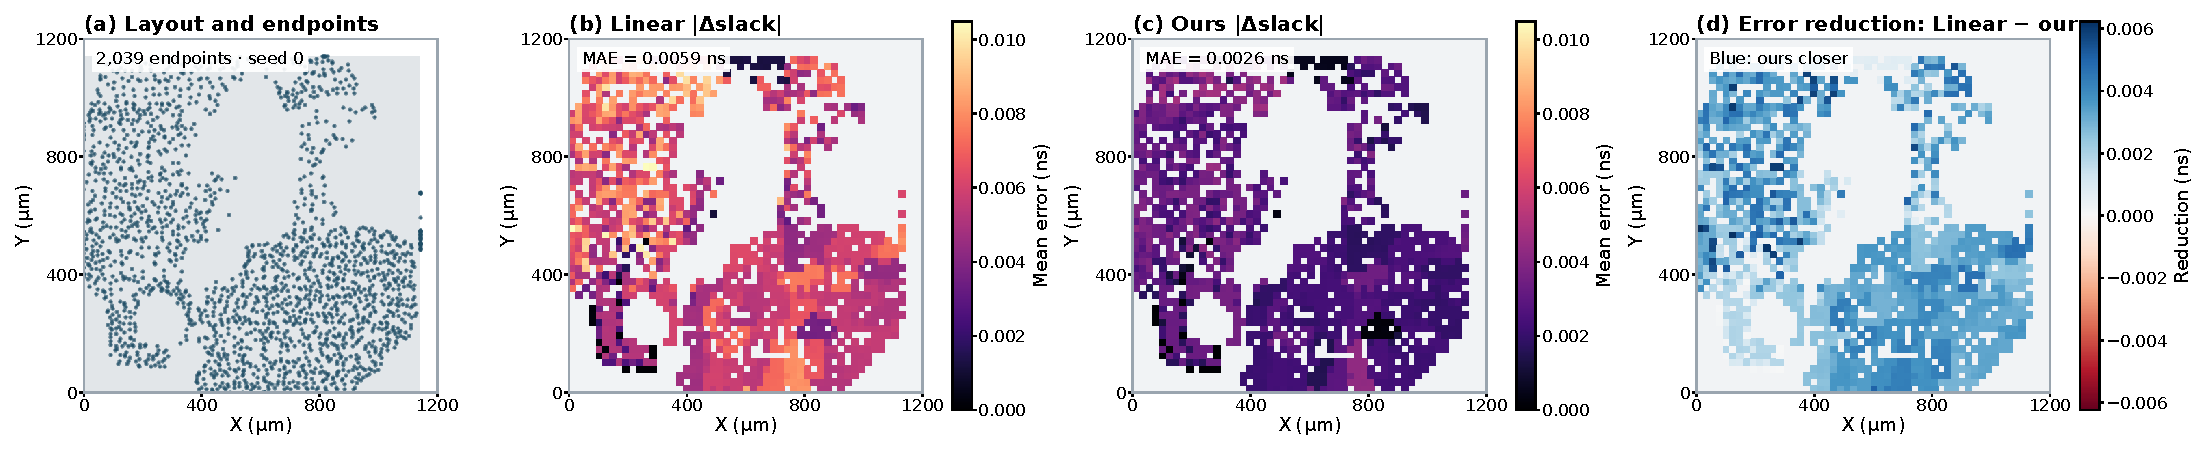
\includegraphics[width=\linewidth]{sta_visualization/gf180_ibex_50/figures/fig_downstream_sta_spatial_row.pdf}
\caption{\textbf{Spatial timing fidelity.} GF180/IBEX, 50\% block mask, seed 0.
Left to right: layout, Linear error, ours, error reduction.
Gray: empty bins; blue: improvement.}
\label{fig:sta-spatial}
\end{figure}

\section{Conclusion}
We study capacitance prediction conditioned on sparse physical observations,
with particular attention to queries beyond their geometric support. A shared
Transformer learns neural corrections and component-wise routing among numerical
and neural proposals relative to an observation-derived anchor.
The method improves over rank-matched CMI in all 15 headline conditions.
Matched-budget learned controls show larger gains from full routing on the
FEM reference than on public rules, with two transfer conditions favoring a
binary gate. Writing predictions into extraction rules lowers capacitance and
worst-slack deviations in all 16 downstream settings. These results support
observation-conditioned residual prediction and a condition-dependent benefit
of hybrid routing; broader extrapolation ranges and other physical responses
remain to be tested. Appendix~\ref{app:limitations} discusses the implications
and limits of the empirical evidence.

\clearpage
\bibliography{references}
\bibliographystyle{iclr2027_conference}
\clearpage
\appendix

\section{Related Work}
\label{sec:related_work}
\label{app:related-work}

\paragraph{Prediction from observation context.}
Conditional Neural Processes learn to predict from observed input--output pairs
and can use a new context set at test time~\citep{garnelo2018cNP}.
Attentive Neural Processes let each query attend to relevant context
points~\citep{kim2019anp}. Our model shares the use of observations as inference
inputs, producing deterministic capacitance estimates conditioned on geometry,
material context and available responses. Its specific design integrates a
support-derived anchor, numerical correction branches and component-wise routing.
We evaluate extrapolation relative to each episode's observed hull as well as
interpolation within it. The contribution lies in this architecture and its
capacitance evaluation; observation-conditioned prediction itself is established
by these prior works.

\paragraph{Learned routing and adaptive combinations.}
Routing Networks learn input-dependent compositions of function
blocks~\citep{rosenbaum2018routing}. RouteLLM learns to select between language
models to balance response quality and inference cost~\citep{ong2025routellm}.
These works establish learned routing as a way to adapt computation to an input.
Our router instead assigns soft weights to corrections for each query and
capacitance component. Its candidates combine deterministic numerical estimators
with two readings of a shared neural residual, all relative to one anchor.
All applicable branches are evaluated in the full model; routing combines their
outputs rather than providing conditional-computation savings. Joint training
uses prediction loss without labels identifying a preferred branch.

\paragraph{Numerical estimators and residual correction.}
PCHIP provides shape-preserving one-dimensional interpolation~\citep{pchip},
and Gaussian-process regression provides kernel-based prediction from observed
values~\citep{gpml}. These estimators supply explicit numerical proposals in our
model; their formulas and boundary conventions appear in
Appendix~\ref{app:classical}. In capacitance modeling, ResCap learns residuals
to a physics-guided initial estimate~\citep{tsai2025rescap}.
Our numerical anchor and analytic proposals are reconstructed from the current
observations. The network learns both a residual and its combination with these
proposals under changing support. The local envelope provides an
observation-based inductive bias; it is not a guaranteed physical bound, and it
does not constrain the neural branch outside support.

\paragraph{Learned capacitance models and extraction.}
OpenRCX reuses process-specific rules derived from characterized wire
patterns~\citep{openrcx}. CNN-Cap learns capacitance from convolutional geometry
representations~\citep{cnncap}. AttentionCap learns capacitance matrices with a
customized Transformer and process-node embeddings, and demonstrates adaptation
to an unseen node through fine-tuning~\citep{attentioncap}.
Our setting makes the current geometry--capacitance observations explicit inputs
and keeps model parameters fixed during target inference. The benchmarks compare
predictors supplied with the same observed support and query coordinates.
They do not establish performance relative to geometry-based extractors on
those methods' original tasks. Export to OpenRCX separately tests how query
prediction errors affect extraction and timing on unchanged layouts.

\section{Structural families and geometric context}
\label{app:structural-families}

The four-way structural-family indicator in Section~\ref{sec:tokens} identifies
the arrangement of the target conductor and its surrounding conductors.
Figure~\ref{fig:structural-families} illustrates the four configurations used to
interpret these labels. The drawings are schematic cross sections: orange
marks the target, blue marks neighboring conductors in the target layer,
green marks a conductor in an upper layer, and gray marks grounded context.
Dielectric regions and outer simulation boundaries are omitted for clarity.
The family name specifies a relative arrangement, while dimensions, layer
indices and material properties are supplied separately by geometry and context.

\begin{figure}[htbp]
\centering
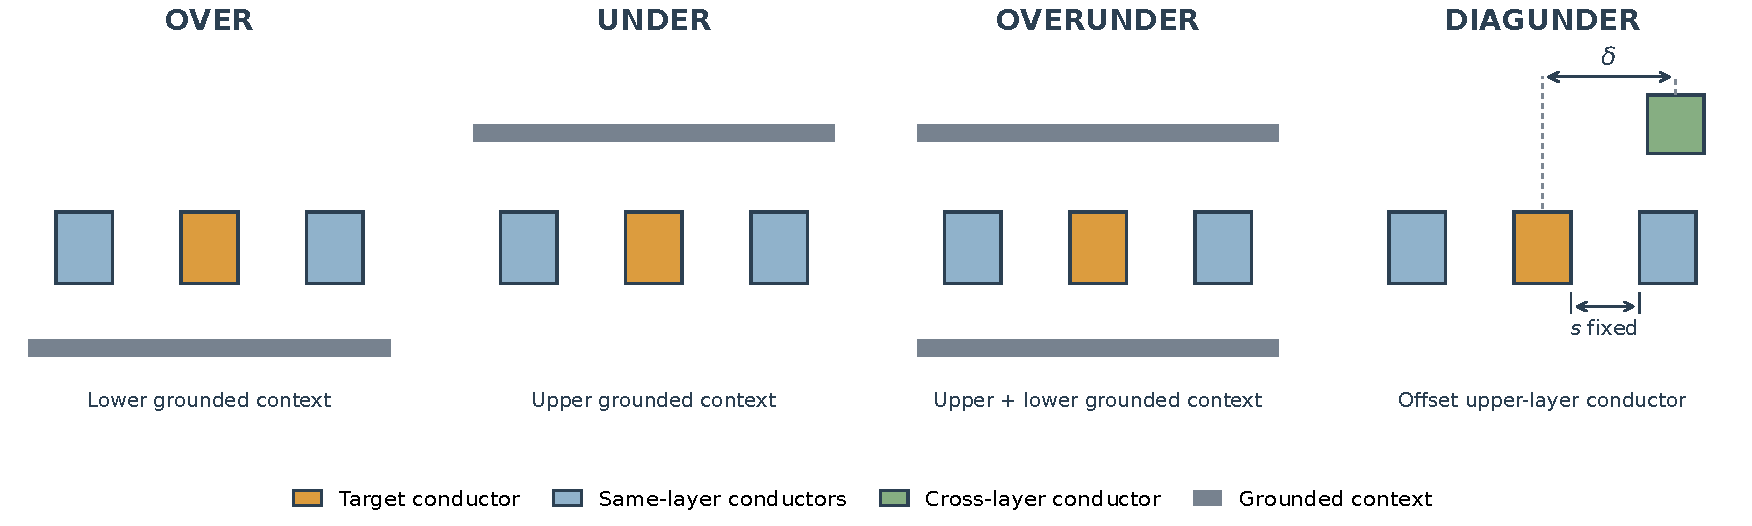
\includegraphics[width=\linewidth]{figure/structural_families.pdf}
\caption{\textbf{Four structural families.} OVER places the target above lower
grounded context; UNDER places it below upper grounded context; OVERUNDER
includes both. DIAGUNDER includes an upper-layer conductor with lateral offset
$\delta$ from the target. In the reference configuration, its same-layer gap
$s$ is fixed while the cross-layer offset varies. Colors identify conductor
roles; the cross sections are not to scale and do not depict the complete
simulation domain.}
\label{fig:structural-families}
\end{figure}

\paragraph{OVER.}
The target and its same-layer neighbors lie above a grounded context conductor.
The configuration includes lateral interaction between same-layer conductors
and coupling to the lower context. ``Over'' refers to the target's position
relative to this lower context.

\paragraph{UNDER.}
The target and its same-layer neighbors lie below a grounded context conductor.
This configuration retains lateral interactions and places the additional
context above the target. ``Under'' refers to this relative vertical ordering.

\paragraph{OVERUNDER.}
Grounded context conductors are present both below and above the target layer.
The target therefore interacts with its lateral neighbors and with context on
both sides vertically. The upper and lower context layers are distinct parts
of the arrangement.

\paragraph{DIAGUNDER.}
An upper-layer signal conductor is laterally displaced from the target, giving
both horizontal and vertical separation. Here ``diagonal'' describes their
relative positions in cross section, not a slanted conductor. In the illustrated
reference family, the same-layer gap remains fixed as the cross-layer offset
changes. This distinguishes offset cross-layer coupling from the planar upper
context shown for UNDER.

\paragraph{Role in conditioning.}
The indicator tells the shared network which arrangement a query belongs to;
it does not encode a process identity or replace the observed capacitances.
The target and context-layer indices, continuous geometry and available material
descriptions supply the remaining physical context. The same family can occur
in different process stacks with different dimensions and response values.
These four schematics describe the families used in this study and do not
exhaust commercial extraction pattern categories.

\section{Network specification and operator settings}
\label{app:network-details}

Table~\ref{tab:network-spec} specifies each member of the released ensembles.
Public models use $K=2$; the reference and transfer models use $K=3$.
Each reported domain has its own three-seed ensemble. The following details
complete the equations in Section~\ref{sec:method}.

\begin{table}[ht]
\centering\small
\caption{Exact per-member network dimensions and stage-2 settings.}
\label{tab:network-spec}
\begin{tabular}{@{}lcc@{}}
\toprule
Quantity & Public ($K=2$) & Reference/transfer ($K=3$) \\
\midrule
Geometry/material token width $17+2K$ & 21 & 23 \\
Shared embedding / encoder width & 64 & 64 \\
Encoder layers / heads / head width & 2 / 4 / 16 & 2 / 4 / 16 \\
Feed-forward hidden width & 256 & 256 \\
Residual head & $64\rightarrow2$ & $64\rightarrow3$ \\
Support/context features $23+d+4K$ & 34 & 38 \\
Agreement features $3K$ & 6 & 9 \\
Router input / hidden / output & $104/32/22$ & $111/32/33$ \\
Correction slots $E$ & 11 & 11 \\
Trainable parameters & 105,604 & 106,384 \\
Initial prior gap $\gamma$ / temperature $\tau$ & $8/0.25$ & $2/0.25$ \\
Stage-2 updates / dropout & $24{,}000/0$ & $12{,}000/0$ \\
\bottomrule
\end{tabular}
\end{table}

\paragraph{Support descriptors.}
The descriptor $s_i$ concatenates: observation density, log nearest distance,
log bracketing extent, inside-support indicator and $K$ log envelope widths;
a five-way indicator (outside, missing width, dense rank-one, dense higher-rank,
sparse/degenerate); support rank, log typical neighbor distance and aligned-width
availability; $d$ directional coverage fractions; $3K$ local variation, slope
and slope-difference channels; and the 11 context fields. Distances use
observed-range-normalized coordinates. Local response statistics use up to the
three nearest observed values divided by $\sigma$. The typical distance is the
median nearest-neighbor distance among distinct support points; the dense
indicator compares local extent with twice that distance. Thus no experimental
mask name or hidden response is supplied to the gate.

\paragraph{Analytic operators.}
The aligned-width operator requires two observations with identical non-width
coordinates to the query and widths bracketing it; its weight is the ordinary
linear fraction between those widths. The six GP operators use reduced
support coordinates $a_j$, query $a_i$, and
\begin{equation}
 f_{\lambda,\rho}(x_i)=\left[\bar y+
 k_i^{\top}(K_{\lambda}+\rho I)^{-1}(Y_S-\mathbf{1}\bar y^{\top})\right]_+,
 \qquad (K_{\lambda})_{jv}=\exp\!\left(-\frac{\|a_j-a_v\|^2}{2L_\lambda^2}\right),
\end{equation}
where $\bar y$ is the observed component mean, $k_i$ is the corresponding
query-to-support kernel vector, and $L_\lambda$ is $\lambda$ times the median
positive pairwise support distance. We use
$\lambda\in\{0.5,1,2\}$ and $\rho\in\{10^{-6},10^{-4}\}$.
Zero-rank support yields a constant proposal; exact observations are restored.
PCHIP is evaluated on sorted rank-one support with the query clamped to its
observed interval. Analytic operators are support-conditioned computations,
not extra pretrained networks.

\paragraph{Numerical conventions.}
All network-side anchors, residuals, envelopes and agreement statistics are
expressed in units of $\sigma$; Eq.~\eqref{eq:main} writes their physical-unit
equivalent. The agreement standard deviation uses a $10^{-12}$ variance floor
for finite derivatives. Invalid branches receive logit $-10^9$ and contribute
nothing to agreement statistics. The model's learned keys are the rows of the
router output projection; descriptor-dependent keys are evaluated separately
in Appendix~\ref{app:routing}. This distinguishes the reported network from
those architectural variants.

\begin{figure}[t]
\centering
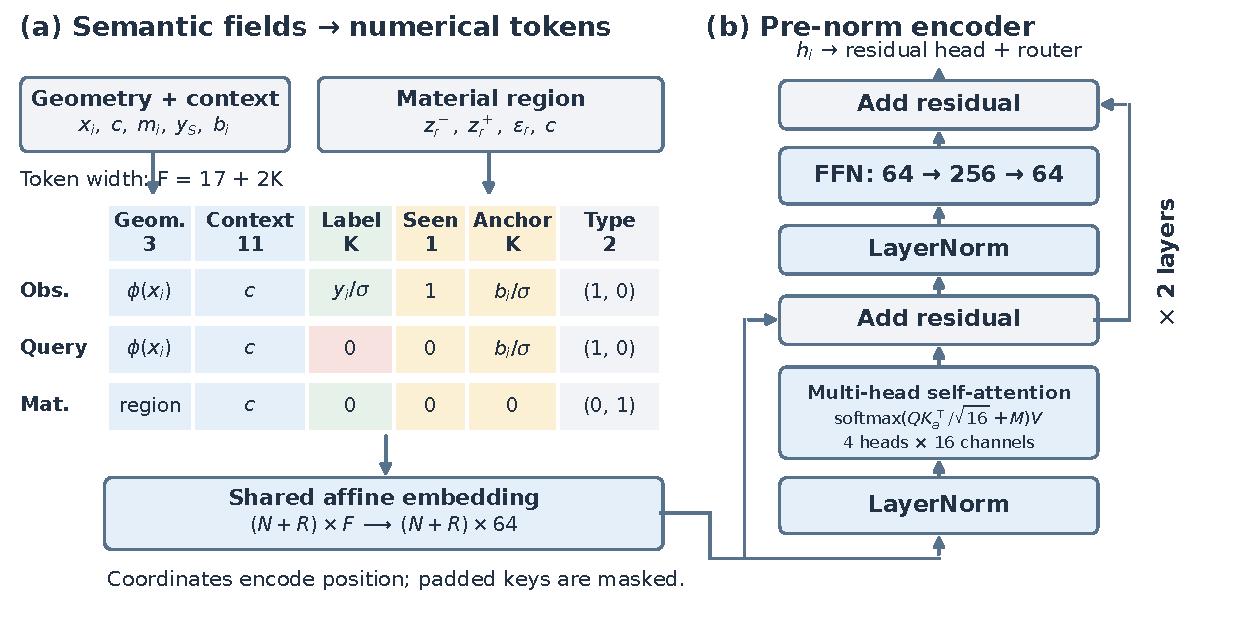
\includegraphics[width=\textwidth]{figure/method_token_encoder.pdf}
\caption{Structured tokenization and the shared encoder. Each geometry row
contains six feature blocks, including an explicit observation indicator;
$\phi(x_i)=\log(1+x_i/\xi)$.
A query retains its geometry and support-derived anchor while its label field
is zero. Material rows encode region extent and permittivity. All valid tokens
participate in attention; two pre-normalized encoder blocks produce one hidden
state per token. Hidden query labels enter only the training loss.}
\label{fig:token-encoder}
\end{figure}

\paragraph{Attention and padding.}
For each head, $Q$, $K_{\!a}$ and $V$ are learned projections of the normalized
token states, and
\begin{equation}
\label{eq:mhsa}
 A=\operatorname{softmax}\!\left(QK_{\!a}^{\top}/\sqrt{16}+M\right),
 \qquad O=AV.
\end{equation}
$M_{ij}=-\infty$ for a padded key and zero otherwise. Head outputs are
concatenated and projected back to width 64; the feed-forward activation is
ReLU. The reported stage-2 models use zero dropout.


\paragraph{Routing sensitivity.}
The coupling can be seen directly from the router's local sensitivity. Holding
branch proposals fixed, when the pre-projection output is positive,
\begin{equation}
\label{eq:gate-gradient}
 \frac{\partial\hat y_{i,k}}{\partial a_{i,e,k}}
 =\frac{\pi_{i,e,k}}{\tau}\left(
 \Delta_{i,e,k}-\sum_{e'\in\mathcal{E}_i}\pi_{i,e',k}\Delta_{i,e',k}\right).
\end{equation}
An update therefore depends on how a proposal changes the current mixture,
weighted by the final prediction error through the chain rule. This trains
routing for the actual query-prediction task without requiring a separate target
that names the best branch.


\begingroup\raggedright
\paragraph{Implementation entry points.}
\label{app:codemap}
In the released study, \texttt{unified/basis.py} constructs support and analytic
corrections; \texttt{unified/episodes.py} builds tokens and padded batches;
\texttt{unified/model.py} implements the encoder, residual head, gate and priors.
Training and warm-start logic are in \texttt{unified/train.py}; inference,
observed-value restoration and pruning are in \texttt{unified/score.py}.
The \texttt{cmi.py}, \texttt{score\_baselines.py}, \texttt{regime.py},
\texttt{aggregate.py} and \texttt{paired.py} modules provide baselines and
metrics. The selection, branch and runtime diagnostics are in
\texttt{scripts/final\_selection.py}, \texttt{score\_elements.py},
\texttt{diagnose\_cells.py} and \texttt{benchmark\_interpolation.py};
\texttt{run\_sta\_visualization.py} reproduces the endpoint audit.
\par\endgroup

\section{Classical estimation}
\label{app:classical}

\begin{figure}[htbp]
\centering
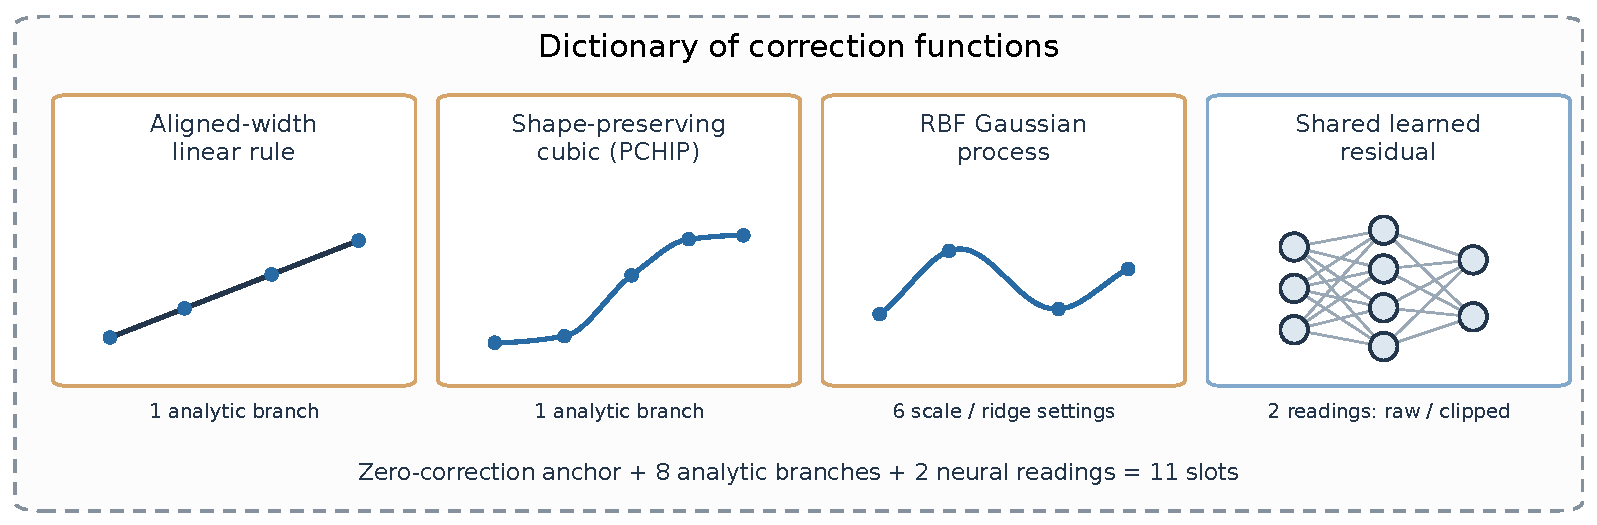
\includegraphics[width=\linewidth]{figure/correction_dictionary.pdf}
\caption{Dictionary of correction functions (schematic). The analytic branches
comprise one aligned-width linear rule, one shape-preserving cubic interpolant,
and six RBF-GP predictors. The shared neural residual supplies raw and locally
envelope-constrained readings. Together with the zero-correction anchor, these
form 11 slots. Analytic predictions enter as $\Delta_{i,e}=f_e(x_i;S,y_S)-b_i$;
inapplicable branches are masked before component-wise routing. Dots denote
observed support; curves illustrate operator behavior, not measured results.}
\label{fig:correction-dictionary}
\end{figure}

We state the numerical estimators using the observed index set $S$ and
component index $k$. These explicit controls do not identify proprietary
commercial interpolation algorithms. In particular, the simplex-linear
anchor below is distinct from the multidimensional CMI baseline.

\paragraph{Linear interpolation and the aligned-width rule.}
For a one-dimensional query bracketed by observed coordinates $x_a<x_b$,
\begin{equation}
\label{eq:classical-linear}
 b_k(x)=(1-t)y_{a,k}+t y_{b,k},\qquad
 t=\frac{x-x_a}{x_b-x_a}.
\end{equation}
Outside the observed interval, Linear extends the nearest endpoint value.
The aligned-width correction uses Eq.~\eqref{eq:classical-linear} with width
as its coordinate, but is applicable only when both bracketing observations
match all non-width query coordinates. Its residual is $f_{\rm width,k}(x)-b_k(x)$.
For support rank $r>1$, let $a(x)$ denote the support-normalized independent
coordinates and $v_0,\ldots,v_r$ the vertices of an enclosing simplex. Then
\begin{equation}
\label{eq:classical-simplex}
 b_k(x)=\sum_{q=0}^{r}\alpha_q y_{v_q,k},\qquad
 a(x)=\sum_{q=0}^{r}\alpha_q a(x_{v_q}),\qquad
 \sum_{q=0}^{r}\alpha_q=1,\quad \alpha_q\geq0.
\end{equation}
Outside the reduced support hull, or if triangulation fails, the anchor copies
the nearest observed value in these coordinates. Rank-zero support gives a
constant estimate.

\paragraph{Shape-preserving cubic interpolation (PCHIP).}
PCHIP~\citep{pchip} uses shape-preserving support slopes $d_{j,k}$ in a
piecewise cubic Hermite interpolant. On $[x_a,x_b]$, with
$\Delta x=x_b-x_a$ and $t$ as in Eq.~\eqref{eq:classical-linear},
\begin{equation}
\label{eq:classical-pchip}
 p_k(t)=h_{00}(t)y_{a,k}+h_{10}(t)\Delta x\,d_{a,k}
       +h_{01}(t)y_{b,k}+h_{11}(t)\Delta x\,d_{b,k},
\end{equation}
where
\begin{equation}
\begin{aligned}
 h_{00}(t)&=2t^3-3t^2+1, & h_{10}(t)&=t^3-2t^2+t,\\
 h_{01}(t)&=-2t^3+3t^2, & h_{11}(t)&=t^3-t^2.
\end{aligned}
\end{equation}
The slopes preserve the local monotonicity of the observed data. Our PCHIP
control clamps queries to the observed interval, extending endpoint values
outside it; the network branch uses sorted rank-one, single-width support.

\paragraph{Inverse-distance weighting (IDW).}
The IDW baseline predicts
\begin{equation}
\label{eq:classical-idw}
 f_{{\rm IDW},k}(x)=\frac{\sum_{j\in S}w_j(x)y_{j,k}}
 {\sum_{j\in S}w_j(x)},\qquad
 w_j(x)=\max\!\left(\|a(x)-a(x_j)\|,10^{-12}\right)^{-2}.
\end{equation}
IDW is an external baseline, not an additional slot in the correction dictionary.

\paragraph{RBF Gaussian-process prediction.}
The mean-centered RBF-GP estimator~\citep{gpml} is
\begin{equation}
\label{eq:classical-gp}
 f_{{\rm GP},k}(x)=\bar y_k+
 \mathbf{k}(x,S)^{\top}(\mathbf{K}+\rho I)^{-1}
 (y_{S,k}-\bar y_k\mathbf{1}),\qquad
 \bar y_k=\frac{1}{|S|}\sum_{j\in S}y_{j,k},
\end{equation}
with $\mathbf{K}_{jv}=\kappa(x_j,x_v)$,
$\mathbf{k}(x,S)_j=\kappa(x,x_j)$, and
\begin{equation}
\label{eq:classical-rbf}
 \kappa(x,x')=\exp\!\left(-\frac{\|a(x)-a(x')\|^2}{2\ell^2}\right).
\end{equation}
Distances use support-normalized independent coordinates. The network's six
GP branches use $\ell=\lambda D_S$, where $D_S$ is the median positive pairwise
support distance, $\lambda\in\{0.5,1,2\}$ and
$\rho\in\{10^{-6},10^{-4}\}$. Their proposals are projected to nonnegative
values before subtracting the anchor, as specified in
Appendix~\ref{app:network-details}. All support computations exclude query
responses, and observed entries are restored exactly at inference.

\section{Why residual initialization and joint routing matter}
\label{sec:ablations}
\label{app:ablations}

\begin{table}[htbp]
\centering
\caption{\textbf{Design choices behind neural--numerical routing.} Validation NRMSE
($\downarrow$). Each panel is a separate controlled comparison, retaining its
recorded validation protocol macro rather than the regime-specific
confirmation scores of Tables~\ref{tab:completion}--\ref{tab:transfer}.
Panel A controls architecture, data and budget; B varies stage-2 updates;
C varies the initial prior of the eight analytic corrections.}
\label{tab:design}\label{tab:ablations}\label{tab:schedule}\label{tab:gap}
\tableinput{main_design.tex}
\end{table}

Table~\ref{tab:design} connects the training procedure to its motivation.
A zero-initialized residual competes with immediately usable numerical
operators, making joint training from scratch a weak starting point.
Initializing the residual first reduces random/block/extrapolation error
from 0.1827/0.2955/0.3767 to 0.1215/0.2050/0.2755 even with a frozen trunk;
subsequent joint training reaches 0.1000/0.1930/0.2755. This supports learning
a useful correction before learning how strongly to use it.

Longer schedules continue to improve the measured validation scores
(panel B), without establishing gains beyond the tested budget.
The initial analytic-branch prior also matters: on the FreePDK15 source-validation
cohort for transfer to ASAP7, changing it from $-8$ to $-2$ lowers all three errors (panel C).
Thus routing depends on both the available corrections and their accessibility
during optimization; adding branches alone does not ensure they are used well.

\paragraph{Anchor-only control.}
On the FEM reference, the anchor-only control isolates the contribution of
residual gating. It already improves on CMI outside support, but residual
gating reduces out-of-support block/extrapolation error from 0.6542/0.5663 to
0.1203/0.1137. For out-of-support random masks, the anchor's 0.0606 is better
than our 0.0895. These internal controls complement the training-stage
ablation in Table~\ref{tab:design}; Tables~\ref{tab:completion} and
\ref{tab:transfer} compare the full model with external methods.

\paragraph{Routing limitations.}
\label{sec:channels}
On ASAP7 out-of-support random masks, the anchor scores 0.0595 compared with
our 0.0877, so the learned mixture does not always improve on its numerical
reference. Descriptor-dependent keys give mixed validation results, and the
validation-selected variant worsens three of five confirmation conditions.
The tested variants and numerical-selector definition are retained in
Appendix~\ref{app:routing}.

\paragraph{Computational cost.}
\label{sec:timing}
The complete three-member ensemble costs about 16$\times$ CMI per query
on 13-node public tables and 3--4$\times$ on 128-node grids on a shared,
single-thread host. The larger query batch amortizes support construction.
Removing eight little-used analytic branches on public rules changes NRMSE by
at most 0.5\% relative and reduces measured scoring time by 6.1$\times$.
This is a separate pruning diagnostic; all headline accuracy comparisons use
the full bank. Appendix~\ref{app:latency} reports the costs and session variation.

\subsection{Matched-budget learned controls}
\label{app:matched-controls}

The earlier direct, residual and binary-gated checkpoints each received only
2,000 updates, and the public versions predate the downstream exclusions.
They therefore do not provide a matched-budget test of the reported model.
We separately train two simpler predictors to distinguish the benefit of
cross-table learning from that of routing:
\begin{align}
 \hat y_i^{\rm residual}&=[b_i+\sigma\odot r_i]_+,\\
 \hat y_{i,k}^{\rm binary}&=[b_{i,k}+\alpha_{i,k}\sigma_k r_{i,k}]_+,
 \qquad 0\leq\alpha_{i,k}\leq1.
\end{align}
The first is an ungated residual Transformer with the same tokens, encoder and
residual head. The second uses a component-wise two-slot softmax over the
anchor and raw neural residual; its gate reads the hidden state and the same
support/context features. Neither includes analytic correction branches or
the clipped neural reading, and the binary gate has no bank-disagreement
features. The latter is a newly trained two-branch model, distinct from
inference-time pruning of the full model to three remaining slots.
These comparisons test the utility of routing under the reported data and
training budget; they do not establish that an ungated neural predictor
cannot represent a similar correction. The full-versus-binary comparison
changes the analytic bank, clipped reading and agreement features together;
it does not separately identify the effect of each of these additions.

For each setting and seed, both controls reuse the full model's fitting tables,
training scales and 2,000-step residual initialization. They retain the same
family-balanced episode sampler, random seed, loss, AdamW settings, gradient
clipping and stage-2 updates: 24,000 for public rules and 12,000 for
reference/transfer. The last checkpoint is used without separate hyperparameter
search for the controls; thus these are controls under the reported training
recipe, not an exhaustive optimization of each smaller architecture.
All reported predictions average three independently trained members.
Each public member has 101,506 parameters for the ungated model, 104,809 for
the binary model and 105,604 for the full model; the corresponding three-output
models have 101,699, 105,196 and 106,384 parameters.

The new evaluations retain the headline 30\% masks, five mask seeds, query
indices, support partition and macro-NRMSE aggregation. Full-model scores are
read from the original reported ensemble records. These supplementary
comparisons use the existing confirmation cohorts; they are not presented as
a newly blinded benchmark. Source-only transfer controls are fitted on eight
FreePDK15 tables and use the inherited source-selected training recipe.

\begin{table}[htbp]
\centering
\caption{\textbf{Matched-budget learning and routing controls.} Confirmation
NRMSE at 30\% missingness. Each row is a three-member ensemble with the same
training data, residual initialization and update budget within its setting.
Bold marks the lowest value; underlining marks our second-best value
in each condition.}
\label{tab:matched-controls}
\tableinput{supp_matched_controls.tex}
\end{table}

\paragraph{Overall and reference-domain comparisons.}
Across the 15 confirmation conditions, the full ensemble improves on the
ungated residual in 14 and on the binary gate in 13. Its advantage is largest
on the two-dimensional FEM reference: it improves all five conditions against
both controls, reducing NRMSE by 18.1--73.3\% relative to the binary gate.
For example, in-support random NRMSE is 0.0103 for the full model, 0.0387 for
the binary gate and 0.0529 for the ungated residual. These differences support
the utility of the full hybrid design under the reference-domain training
recipe, rather than attributing all gains to cross-table learning alone.

Transfer to ASAP7 is less uniform. Full routing improves on the ungated
residual in all five conditions, but the binary ensemble is better on
out-of-support block masks (0.1291 versus 0.1358) and extrapolation masks
(0.1037 versus 0.1073). The full branch bank is consequently not a uniformly
better choice across the evaluated settings.

\paragraph{Public-rule attribution.}
The full ensemble has lower point estimates than the binary gate in all five
public conditions, but the relative improvements range from only 0.6\% to
5.6\%. The ungated residual has a lower point estimate for in-support block masks
(0.0645 versus 0.0678), while the full model is better in the other four
conditions. Much of the reduction relative to numerical interpolation is
therefore already achieved by a support-conditioned residual Transformer.

Table~\ref{tab:control-bootstrap} qualifies the small routing gains. The full
model's paired intervals exclude zero against the binary gate in the two
in-support conditions, but not in any of the three out-of-support conditions.
Against the ungated residual, they exclude zero in favor of the full model
for in-support random and out-of-support block masks. These are pointwise
comparisons conditional on the trained ensembles, not evidence of a uniform
advantage across training seeds or a guarantee that the full branch bank is
necessary. Together with the pruning diagnostic, the public evidence supports
a strong learned residual and more limited gains from the extra routing machinery.

\paragraph{Training-seed checks and interpretation.}
Replaying all original full-model members reproduces the reported ensemble
NRMSEs exactly in all 15 conditions. Comparing corresponding individual seeds,
the full model beats the ungated residual in 12/15 public, 15/15 reference and
13/15 transfer seed--condition pairs; against the binary gate the counts are
9/15, 13/15 and 13/15. These descriptive counts are not independent statistical
tests. They also need not match ensemble win counts, because averaging
predictions precedes computing ensemble NRMSE. The reference advantage is
stronger than the public advantage, but neither seed counts nor pooled
ensemble scores establish uniform dominance. In particular, these controls
support a condition-dependent benefit of the full hybrid design, not the
necessity of every analytic operator in every domain.


\begin{table}[htbp]
\centering
\caption{\textbf{Paired public-group uncertainty for the routing controls.}
Difference is full routing minus the named comparator, so negative favors the
full model. Pointwise 95\% intervals use 2,000 paired group-bootstrap samples,
retaining all masks of each dependency group. The intervals condition on the
trained ensembles and are not multiplicity-adjusted.}
\label{tab:control-bootstrap}
\tableinput{supp_control_bootstrap.tex}
\end{table}


\subsection{An extrapolation-capable numerical control}
\label{app:affine-control}

To distinguish learned gains from endpoint-clamping conventions, we add a
local affine predictor that continues its fitted trend beyond the support hull.
Coordinates are normalized by the observed range and projected onto the
independent axes of the observed support. For each query, the predictor fits
an affine function to its $m$ nearest observed points, using at least $r+1$
points when available, where $r$ is the support rank:
\begin{equation}
 (a_i,B_i)=\arg\min_{a,B}\sum_{j\in N_m(i)}
 \|y_j-a-B(z_j-z_i)\|_2^2+10^{-8}\|B\|_F^2,
 \qquad \hat y_i=[a_i]_+.
\label{eq:local-affine-control}
\end{equation}
The intercept is unpenalized; rank-zero support returns its mean response.
The predictor preserves observed entries exactly. It does not clip predictions
to endpoint values or a local response envelope.

We select $m\in\{2,4,8,16\}$ by the mean of the five defined
regime/protocol validation NRMSEs at 30\% missingness, using the original five
mask seeds. The public validation pool has the same downstream exclusions as
the reported public model; the transfer validation pool contains FreePDK15
only. The selected counts are 4 for public rules and 8 for reference and
transfer. Selection is recorded before scoring confirmation. Confirmation
uses exactly the query indices, support regions, truth-energy accumulators
and normalization scales of the headline comparisons.

\begin{table}[htbp]
\centering
\caption{\textbf{Local affine extrapolation versus the support anchor and full
model.} Confirmation NRMSE at 30\% missingness; lower is better.
The affine predictor can extrapolate outside support and its neighbor count
is selected only on validation. Bold marks the lowest value; underlining marks our second-best value
in each condition.}
\label{tab:affine-control}
\tableinput{supp_affine_control.tex}
\end{table}

The full model is better than this extrapolation-capable control in 13 of 15
conditions. On public out-of-support block and extrapolation masks, the
comparison changes from 0.5588/0.6503 to 0.1391/0.1620. Thus the gains in these
conditions do not depend solely on comparing against endpoint extension.
However, local affine prediction is better on out-of-support random masks
for both the FEM reference (0.0621 versus 0.0895) and transfer to ASAP7
(0.0594 versus 0.0877). The existing anchor failures therefore remain material;
the learned mixture does not uniformly improve extrapolation.


\section{Routing diagnostics and alternative gates}
\label{app:routing}

\paragraph{What the numerical branches provide.}
Table~\ref{tab:elements} retains the numerical-operator diagnostic, whose
scope is narrower than a full-network oracle. The scoring script constructs
the anchor and eight analytic corrections without loading neural predictions.
Its label-informed selector chooses a single proposal per query by minimizing
the sum of absolute errors in training-normalized component units; undefined
corrections revert to the anchor in this diagnostic. It is evaluated using
macro NRMSE, a different objective. Thus it is neither an NRMSE lower bound
nor an oracle over all eleven branches or component-wise convex mixtures.
Individual operators are scored only where applicable, so the best-operator
column can also have a different population.

On public out-of-support
random masks, the network's 0.0910 is well below the numerical selector's
0.4297, illustrating the contribution unavailable to this diagnostic.

\begin{table}[htbp]
\centering
\caption{\textbf{Numerical-operator diagnostics at 30\% random missingness.}
NRMSE ($\downarrow$). Best operator* is scored on its applicability subset;
parentheses identify the operator. The label selector reads query truth,
uses only numerical branches and is not a deployable method or a bound
on the full network. Other columns use the full query population.
Bold marks the lowest displayed NRMSE; underlining marks the second-lowest
displayed Ours value. Populations and label
access differ as described above.}
\label{tab:elements}
\tableinput{supp_operators.tex}
\end{table}

\paragraph{Descriptor-dependent keys.}
We tested five-channel descriptor keys with pointwise or per-condition
objectives and a six-channel variant whose envelope descriptor also covers
outside-support queries. Table~\ref{tab:keyvariant} groups all reported
validation rows by cohort; absent variant/cohort combinations are not inferred.
The descriptor-key variants give mixed results on the source-validation
cohort for transfer to ASAP7.
On the reference and public cohorts, none of the tabulated variants improves
over the reported gate. Boldface reflects numerical comparisons directly.

The source-validation minimax rule ranked a descriptor-key configuration
first for transfer to ASAP7. Its one-time confirmation evaluation worsened three of five conditions,
including out-of-support random NRMSE (0.107 versus 0.088). We retain the
headline configuration fixed before these exploratory variants, and do not
claim that validation selection identified this failure in advance.

\begin{table}[htbp]
\centering
\caption{\textbf{Descriptor-key validation diagnostics at 30\% missingness.}
NRMSE ($\downarrow$), grouped by cohort. Bold marks the lowest NRMSE
among all gates in each cohort/condition; underlining marks our second-best
value. All available rows are retained.
The transfer row uses only FreePDK15 source-validation tables, not ASAP7 labels.}
\label{tab:keyvariant}
\tableinput{supp_keyvariants.tex}
\end{table}

\section{Latency and evaluated branch pruning}
\label{app:latency}

Table~\ref{tab:latency} combines the original method comparison and the
later platform breakdown. Both use interleaved execution on a shared host,
with one BLAS thread and one PyTorch thread. One episode is one table's
query set: six queries for the 13-node public workload and 64 for the
128-node reference workload. The full three-seed ensemble includes support
construction, numerical branches and Transformer passes.

The platform session gives ratios of 15.77--16.41$\times$ CMI for public
rules and 3.06$\times$ for the ASAP7 reference grid. Repeating the original
benchmark unchanged gives 16.07$\times$/3.05$\times$, compared with
15.96$\times$/4.03$\times$ in its recorded session. Hence we report a
3--4$\times$ reference range; absolute times and fine differences depend on
shared-host load. These measure query-prediction costs, not field-solver speedups.

\begin{table}[htbp]
\centering
\caption{\textbf{Single-thread query-prediction cost.} Panel A retains the original
full-method timing comparison; panel B pairs CMI with the full ensemble by
platform in a separate session. The latter retains median query latency and
P95 episode latency without repeating equivalent batch/table columns.
CMI ratios use unrounded timings; the two sessions should not be pooled.
Bold marks the minimum per table class and metric in panel A, and the
lower CMI/ours latency in each platform/workload pair in panel B.
Underlined Ours timings rank second within the corresponding comparison.}
\label{tab:latency}\label{tab:timing}\label{tab:costplatform}
\tableinput{supp_runtime.tex}
\end{table}

\paragraph{Pruning diagnostic.}
On public rules, removing PCHIP, aligned-width interpolation and six GP
branches changes in-support random/block NRMSE from 0.0803/0.0678 to
0.0804/0.0678, and out-of-support random/block/extrapolation from
0.0910/0.1391/0.1620 to 0.0912/0.1398/0.1628. The largest relative change
is below 0.5\%, while the measured scoring pipeline is 6.1$\times$ faster.
This diagnostic follows observed gate usage and includes recomputation of
agreement features; it is not used to replace the full-bank headline results
or to claim the same saving on rank-two tables.

\section{Dataset organization and construction}
\label{app:data-construction}

The benchmark organizes characterized geometry--capacitance pairs into
observation-conditioned prediction episodes. Its construction combines public
extraction rules, independently solved numerical grids and controlled masks.
Table~\ref{tab:data-overview} summarizes the data used by the different protocols.
The contribution is this organization and evaluation interface together with the
numerical reference; the public rule values originate from existing process
resources.

\begin{table}[htbp]
\centering\small
\caption{\textbf{Data and evaluation cohorts.} Counts describe the indicated
protocols, not additive counts of independent datasets. Public split counts are
the original allocation before the downstream exclusions described below.
Boundary cohorts supplement the headline confirmation evaluations.}
\label{tab:data-overview}
\begin{tabular}{@{}>{\raggedright\arraybackslash}p{0.19\linewidth}>{\raggedright\arraybackslash}p{0.26\linewidth}>{\raggedright\arraybackslash}p{0.47\linewidth}@{}}
\toprule
Data / protocol & Geometry and responses & Size and use \\
\midrule
Public rules & Rank-one variation; $K=2$ &
1{,}713 tables across ASAP7, GF180, IHP-SG13G2 and Sky130; original
train/validation/test allocation: 1{,}116/256/341; 340 scored test instances
after duplicate weighting. \\
\addlinespace
Numerical reference & Rank-two width--distance grids; $K=3$ &
27 evaluation tables, each $8\times16$ geometries: 16 confirmation,
8 validation and 3 boundary-layer tables. Fitting uses 16 separate
$9\times17$ tables; configuration selection uses 24 validation tables. \\
\addlinespace
ASAP7 transfer & Target observations, frozen source parameters &
8 new-geometry confirmation tables; 2 boundary-layer tables evaluated separately. \\
\addlinespace
Downstream audit & Fixed routed layouts; masked extraction rules &
84 rewritten tables excluded from model fitting; 16 process/design/mask
settings on 8 fixed layouts. \\
\bottomrule
\end{tabular}
\end{table}

\subsection{Public rule-table organization}
The public corpus contains 1{,}713 capacitance tables from ASAP7, GF180,
IHP-SG13G2 and Sky130 extraction rules. A row stores a candidate wire geometry
and its capacitance response vector. Tables carry the structural families
OVER, UNDER, OVERUNDER and DIAGUNDER, together with the available layer and
material context used by the tokenizer in Section~\ref{sec:tokens}.
Public models predict two response components ($K=2$).

The original partition assigns associated groups to training, validation and
test, yielding 1{,}116, 256 and 341 tables, respectively. Duplicate weighting
leaves 340 scored test instances. These original counts must be distinguished
from the exclusions made for the downstream audit. Although three coordinates
are stored, every public table has one constant coordinate and two identical
varying coordinates. We verified this property across all 1{,}713 tables;
observed support is rank one under the evaluated masks. The rank-matched
multilinear control is therefore CMI-1D. The rule responses are extraction
references, rather than independent field-solver truth.

\subsection{Independent numerical reference and transfer}
The numerical reference comprises 27 tables constructed from ASAP7 and FreePDK15
CTF material descriptions. Each table samples an $8\times16$ grid in wire width
and distance, giving 128 candidate geometries. Capacitances are computed under
unit conductor excitations using quadratic finite elements~\citep{skfem} on
Gmsh meshes~\citep{gmsh}. The resulting grids span two independent geometric
axes and use three response components ($K=3$); their rank-matched baseline is
CMI-2D. The construction is a two-dimensional physical idealization.

Sixteen tables provide new-geometry confirmation, eight provide validation,
and three form a boundary-layer cohort. These 27 tables contain no training partition: the headline reference
confirmation and boundary results come from this collection, whereas fitting
and model selection use the separate cohorts specified below. Source-only
transfer trains on FreePDK15 tables and evaluates new geometries on ASAP7. The reported
target is ASAP7, with eight confirmation tables and a separate two-table
boundary cohort. Target observations enter the support computations and model
inputs, but they never trigger target-domain parameter updates. Source training
scales remain fixed. Model selection also uses source labels only: the
12 tables in the archived \texttt{to\_asap7\_val} cohort are all FreePDK15.
The earlier labels ``To ASAP7 val.'' denote the transfer destination, not the
process supplying validation labels. This applies to the branch-prior and
alternative-gate comparisons in Tables~\ref{tab:design} and~\ref{tab:keyvariant}.
Appendix~\ref{app:boundary} reports the small boundary cohorts separately from
the headline results.

\paragraph{Fitting and selection cohorts.}
The original FEM collection contains 32 tables on $9\times17$ grids
(153 geometries per table), split into 16 training, eight validation and eight
original test tables across the two processes. Reference fitting uses the
16 training tables: four structural families at layer indices 2 and 3 in each
process. The stage-1 residual checkpoints and stage-2 models use this same
training partition. The reference model-selection cohort contains 24 tables:
eight original validation tables, eight second-round validation tables, and
eight validation tables from the 27-table collection. These are layer indices
4 and 6; the two layer-6 collections have different grids. Headline confirmation
uses the 16 third-round tables at layer indices 7 and 8, while the three
boundary tables use indices 1 or 9. Training and headline reference confirmation
have no overlapping process/family/layer/context tuples.

For transfer to ASAP7, stage 1 and stage 2 fit only the eight FreePDK15
training tables. Stage 1 uses four original FreePDK15 validation tables;
subsequent configuration comparisons use 12 FreePDK15 validation tables
(four from each of the three validation collections above). Although the
archived fold file also stores ASAP7 rows marked \texttt{test}, both fitting
loops filter the \texttt{train} partition; those target labels do not enter
updates. Confirmation uses eight ASAP7 tables at indices 7 and 8, and the
two boundary tables use indices 1 and 9. Target observations are read only as
inference context, and withheld target responses are used only for scoring.
The provenance audit checks the cohort hashes in the archived validation
receipts, rather than inferring label access from run names.

\begin{table}[htbp]
\centering\small
\caption{\textbf{Fitting, selection and headline confirmation.} Counts are
unique tables; validation can contain different grids for the same layer.
The public counts reflect downstream exclusions and deduplication.
FEM fitting grids have 153 nodes; the headline FEM/transfer confirmation grids
have 128 nodes. Boundary cohorts are excluded from the last column.}
\label{tab:fit-selection-audit}
\begin{tabular*}{\linewidth}{@{\extracolsep{\fill}}lrrrl@{}}
\toprule
Setting & Fitting & Selection & Confirmation & Selection-label source \\
\midrule
Public rules & 1,051 & 246 & 340 & Public training-domain processes \\
FEM reference & 16 & 24 & 16 & ASAP7 and FreePDK15 \\
Transfer to ASAP7 & 8 & 12 & 8 & FreePDK15 only \\
\bottomrule
\end{tabular*}
\end{table}

\subsection{Support--query episode construction}
For each table, we retain the candidate coordinates $X$ and context $c$, select
observed indices $S$, and assign the remaining indices to $\mathcal Q$.
Only $y_S$ is exposed to the predictor. Query response fields are zeroed before
embedding, with explicit observation indicators distinguishing unavailable
responses from measured zeros. Anchors, envelopes, numerical corrections and
routing descriptors are all reconstructed from the retained observations.
Withheld responses enter only the training loss or evaluation metric.

Evaluation uses random, contiguous-block and boundary-extrapolation masks at
10/30/50/70\% missingness, with five mask seeds and every applicable whole-width
fold. Random masks remove individual observations; block masks remove contiguous
coverage; boundary masks withhold geometries beyond the retained observed range.
Whole-width folds withhold all rows at an applicable width. These masks expose
different support configurations without changing the underlying reference
responses. Training draws fresh masks and missingness rates as specified in
Section~\ref{sec:training}.

After masking, each query is classified by its position relative to the observed
convex hull and affine span. Queries inside this region contribute to the
in-support regime; other queries contribute to the out-of-support regime.
Boundary-extrapolation masks have no in-support queries. The query coordinates
and reference responses still belong to the characterized dataset, so this
protocol measures extrapolation beyond current observations, not unrestricted
extrapolation beyond all characterized geometries. All methods are scored on
the same query population. Validation selects configurations before the
confirmation cohorts are evaluated; Section~\ref{sec:metrics} defines selection
and aggregation. Appendix~\ref{app:surface} reports the 60 populated
cohort--regime--protocol--rate conditions.

\subsection{Separation from downstream extraction data}
The downstream audit writes predictions into 84 masked rule tables and reruns
PEX and STA on fixed routed layouts. Of these 84 tables, 55 belonged to the
original training split. The public ensemble was therefore retrained with all
84 excluded from training, validation and test. Public confirmation results and
the downstream audit use that held-out model family on distinct table
populations. Export preserves unmasked values exactly; the original full-table
extraction supplies the downstream reference. Appendix~\ref{app:downstream}
details the export checks and replay protocol.

This characterization benchmark differs from design-level corpora such as
CircuitNet~2.0~\citep{circuitnet2}, which provide routability, timing and power
data. Our table-level protocols test support-conditioned capacitance prediction;
the separate layout audit tests its consequences for extraction and timing.

\section{Additional prediction evidence}
\label{app:surface}

\subsection{The complete missingness surface}
Table~\ref{tab:surface} places all 60 scored cohort--regime--protocol--rate
conditions in one matrix, pairing our result with rank-matched CMI at each
rate. We improve in all 60 cells.
On the reference, the relative block-mask in-support gain grows from 24\%
at 10\% missingness to 91\% at 70\%, consistent with greater benefit when
contiguous masking removes local interpolation support. At 10\% public
missingness, the evaluated masks remove the same single node, so protocol
scores coincide; these repeated values are not independent evidence.

\begin{table}[htbp]
\centering
\caption{\textbf{Complete missingness surface.} Mean-mask macro NRMSE
($\downarrow$); bold marks the better result in each Ours/CMI pair.
CMI is 1D for public rules and 2D otherwise. All 60 populated conditions
are included; boundary-extrapolation masks have no in-support queries.}
\label{tab:surface}\label{tab:surfacetransfer}
\tableinput{supp_surface.tex}
\end{table}

\subsection{Boundary-layer cohorts}
\label{app:boundary}
Table~\ref{tab:boundary} combines the reference and ASAP7 transfer boundary
cohorts. The method leads all five reference conditions and four of five
ASAP7 conditions; RBF-GP wins ASAP7 in-support random missingness.
These cohorts contain only three and two tables, respectively, so conditions
within a cohort do not establish independent-geometry confidence.

\begin{table}[htbp]
\centering
\caption{\textbf{Boundary-layer prediction at 30\% missingness.}
NRMSE ($\downarrow$), with cohort table counts in parentheses.
Bold marks the best method; underlining marks our second-best value
in each cohort/condition.}
\label{tab:boundary}\label{tab:bnd_reference}\label{tab:bnd_asap7}
\tableinput{supp_boundary.tex}
\end{table}

\subsection{Public-rule uncertainty and process/mode detail}
\label{app:public-detail}
The paired bootstrap keeps all masks of each associated group together and
uses 2,000 replicates. In-support differences (ours minus PCHIP) over 338
groups are $-0.0267$ $[-0.0344,-0.0177]$ for random and $-0.1213$
$[-0.1748,-0.0684]$ for block masks. Out-of-support differences against
CMI-1D over 340 groups are $-0.4622$ $[-0.6010,-0.3955]$,
$-0.8155$ $[-1.0006,-0.4973]$ and $-1.0247$ $[-1.3058,-0.5493]$
for random, block and extrapolation. Every comparison has bootstrap
$P(\mathrm{better})=1.000$.

Table~\ref{tab:modes} retains the process/family breakdown without replacing
the main macro metric. ASAP7 has the highest pooled error in every populated
mode; DIAGUNDER is especially difficult on ASAP7 and Sky130. The IHP
DIAGUNDER cell has no positive truth energy and is absent, rather than zero.
Best/worst summarize individual tables, average gives the mean table RMSE,
and pooled weights queries equally; differences between average and pooled
reflect their weighting conventions.

\begin{table}[htbp]
\centering
\caption{\textbf{Public-rule errors by process and coupling mode.}
30\% block missingness, shown as count:normalized RMSE. Counts denote tables
for best/worst and scored queries for average/pooled, and repeat across
statistics. ``--'' indicates no positive truth energy. Bold marks the lowest
error across processes for each statistic and coupling mode.}
\label{tab:modes}
\tableinput{mode_stats.tex}
\end{table}

\section{Downstream audit protocol and endpoint evidence}
\label{app:downstream}

Table~\ref{tab:downstream} reports all 16 design/process/mask conditions.
Each run reuses the golden routed snapshot and constraints and reruns only
extraction and the final timing report. Golden replay is checked for identical
parasitics; export validation checks both exact preservation of unmasked
lines and round-trip recovery of written values. Mask construction follows
the deterministic table-evaluation recipe, but the 84 rewritten tables are
distinct from the public confirmation cohort and excluded from model fitting.

Worst slack uses each platform's Liberty time unit converted to ns. The
main timing columns take the maximum absolute deviation across the three
seeds for each design and mask. Extraction wall time and peak memory
measure the reporting flow and are not substitutes for query-prediction latency.

\subsection{Endpoint, spatial and decision-level audit}
\label{app:sta-spatial}

We replay the seven existing gf180/ibex SPEFs (one golden and Linear/ours
for seeds 0, 1 and 2 at 50\% block missingness). Each replay reads the same
final connected ODB, the original SDC and the same TC Liberty library using
the pinned OpenROAD/OpenSTA executable. The original routed-database and
constraint hashes agree across the archived runs; SPEF hashes are checked
before loading, and exported cell and port coordinates agree exactly across
all seven replays. Resistance NRMSE is zero in each archived SPEF comparison.
The replays reproduce every archived WS/TNS value within its reported rounding
precision. Aggregating the original records recovers
Table~\ref{tab:downstream}: Linear/ours capacitance NRMSE
0.0199/0.0061, maximum $|\Delta\mathrm{WS}|$ 0.1328/0.03701\,ns and maximum
$|\Delta\mathrm{TNS}|$ 168.6/50.22\,ns. These are three-seed aggregates,
whereas the spatial maps in Figure~\ref{fig:sta-spatial} depict seed 0 alone.

For endpoint $i$, let $E_i^m=|s_i^m-s_i^{\mathrm{gold}}|$ and
$G_i=E_i^{\mathrm{Linear}}-E_i^{\mathrm{ours}}$.
The spatial maps average these errors in identical $50\times50$ bins, using
shared color limits for the two methods and a symmetric scale for $G_i$.
All endpoint coordinates refer to the unchanged physical database.
In Figure~\ref{fig:sta-spatial}, boxes denote placed cells and points denote
constrained endpoints, not routed-metal geometry. Coordinates are in $\mu$m
and errors in ns; the two error maps share color limits, and the difference
map uses a symmetric scale. Gray bins contain no constrained endpoints.

\paragraph{Endpoint coverage and units.}
OpenSTA enumerates 3,859 endpoints in every replay: 2,039 have finite setup
slack and 1,820 are unconstrained. No endpoint is absent from any variant.
The unconstrained endpoints remain in the raw data with infinite slack and
are explicitly excluded from the finite-error, ranking and sign statistics.
For every constrained endpoint we use its minimum setup slack; internal pins
are mapped to their instance's bounding-box center, and output ports to their
physical pin-box center. All coordinates come from ODB in $\mu$m, and all
slacks are in ns. The exported STA properties have $10^{-6}$\,ns display
resolution; a $2\times10^{-6}$\,ns tolerance defines ties only for the fraction
of endpoints with improved error. Violation classification uses the original,
unshifted threshold $s<0$.

\paragraph{Decision definitions.}
A false negative (FN) is a golden violation classified as safe; a false positive
(FP) is a golden-safe endpoint classified as violating. Sign accuracy counts
both correctly safe and correctly violating endpoints. For Top-$K$ agreement
we retain one worst setup path per constrained endpoint, sort by slack with
endpoint/startpoint names breaking ties, and compare either the endpoint sets
(EP@K) or the full ordered data-pin sequences (Path@K). Each overlap is the
intersection size divided by $K$. We also export startpoint--endpoint pair
overlap; it agrees with full-pin-sequence overlap at the reported $K$ values
in this case. Spearman $\rho$ and Kendall $\tau$ use all finite endpoint slacks.

\begin{table}[htbp]
\centering\small
\caption{\textbf{Decision fidelity for all three seeds.} gf180/ibex,
50\% block missingness; 2,039 constrained endpoints per row. MAE and RMSE are
endpoint-slack errors in ns, Sign is slack-sign accuracy, EP@50 is endpoint
overlap, Path@50 uses the full data-pin sequence, and $\rho$ is Spearman
correlation with golden slack. Bold marks the best value within each seed
(lower MAE/RMSE/FN/FP; higher Sign/EP@50/Path@50/$\rho$); ties are bolded.
Our second-best values are underlined. No seed is omitted.}
\label{tab:sta-decision}
\tableinput{sta_decision_fidelity.tex}
\end{table}

Seed 0 improves endpoint error at 99.90\% of endpoints, and seed 1 at
100\%. Seed 2 improves 51.10\%, worsens 48.85\%, and ties on 0.05\%;
its MAE rises from 0.00384 to 0.00396\,ns while RMSE falls from
0.00443 to 0.00416\,ns. The seed-1 endpoint MAE falls from 0.08787 to
0.02610\,ns. At $K=100$, seed-1 endpoint overlap increases from 0.74 to
0.98 and full-path overlap from 0.42 to 0.98. Seeds 0 and 2 have perfect
overlap for both methods at $K=10,20,50,100$. These distinctions matter:
restoring slack values, restoring their ordering and preserving their signs
are related but not interchangeable claims.

\paragraph{Reproducible artifacts.}
The replay script saves input hashes, STA logs, raw endpoint/path exports,
seed-wise CSVs and PDF/SVG/PNG figures; its entry point is listed in
Appendix~\ref{app:network-details}. Additional
scatter and bin-maximum maps expose spatial averaging. No retraining,
rerouting, constraint shifts or ECO operations are used.


% \begin{figure}[p]
% \centering
% 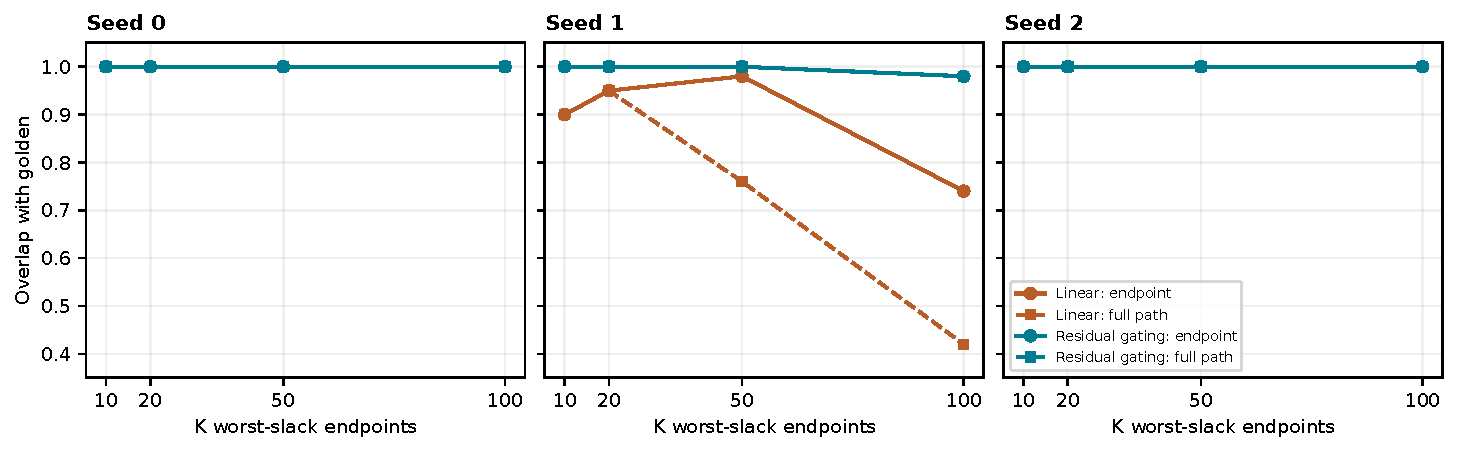
\includegraphics[width=\textwidth]{sta_visualization/gf180_ibex_50/figures/fig_sta_overlap_all_seeds.pdf}
% \caption{\textbf{Critical-set fidelity on GF180/IBEX, 50\% block missingness.}
% Endpoint and full-data-pin-sequence Overlap@$K$ for every seed.
% Both methods recover golden sets for seeds 0 and 2 (curves overlap);
% at $K=100$, seed-1 endpoint/path overlap improves from 0.74/0.42 to
% 0.98/0.98. The database, constraints, Liberty, corner, resistance model
% and STA executable are fixed throughout. Figure~\ref{fig:sta-spatial}
% shows the corresponding seed-0 spatial context and error maps.}
% \label{fig:sta-all-seeds}
% \end{figure}


\subsection{Spatial fidelity across additional process/design settings}
\label{app:sta-additional-spatial}

Figures~\ref{fig:sta-spatial-asap7-ihp} and~\ref{fig:sta-spatial-gf180-sky130}
extend Figure~\ref{fig:sta-spatial} to four additional archived settings:
ASAP7/IBEX, IHP-SG13G2/IBEX, GF180/AES and Sky130HS/IBEX.
All use 50\% block missingness and seed 0, fixed across settings rather than
selected separately by error. The plots are reconstructed from existing STA
exports; no training, routing or timing rerun is introduced.
Golden, Linear and ours have identical endpoint coverage and exported geometry
within each setting. Only endpoints with finite slack in all three variants
are plotted: 3,704, 3,704, 691 and 3,975, respectively.
The archived worst slack and total negative slack are checked against the
endpoint exports before plotting. ASAP7 values are converted from ps to ns;
the other exports already use ns.

Each column follows the four-panel organization of Figure~\ref{fig:sta-spatial}.
Errors are averaged in $50\times50$ spatial bins, with a shared zero-based scale
for Linear and ours within each setting. Error-reduction maps use a symmetric
scale; gray bins contain no constrained endpoints. Color limits and physical
extents vary across settings, so cross-setting comparisons must use the
labeled units rather than color intensity alone. Panel annotations report
endpoint-weighted MAE, not an unweighted average of occupied bins.
These fixed-seed maps supplement the three-seed aggregate audit in
Table~\ref{tab:downstream}.

\begin{figure}[p]
\centering
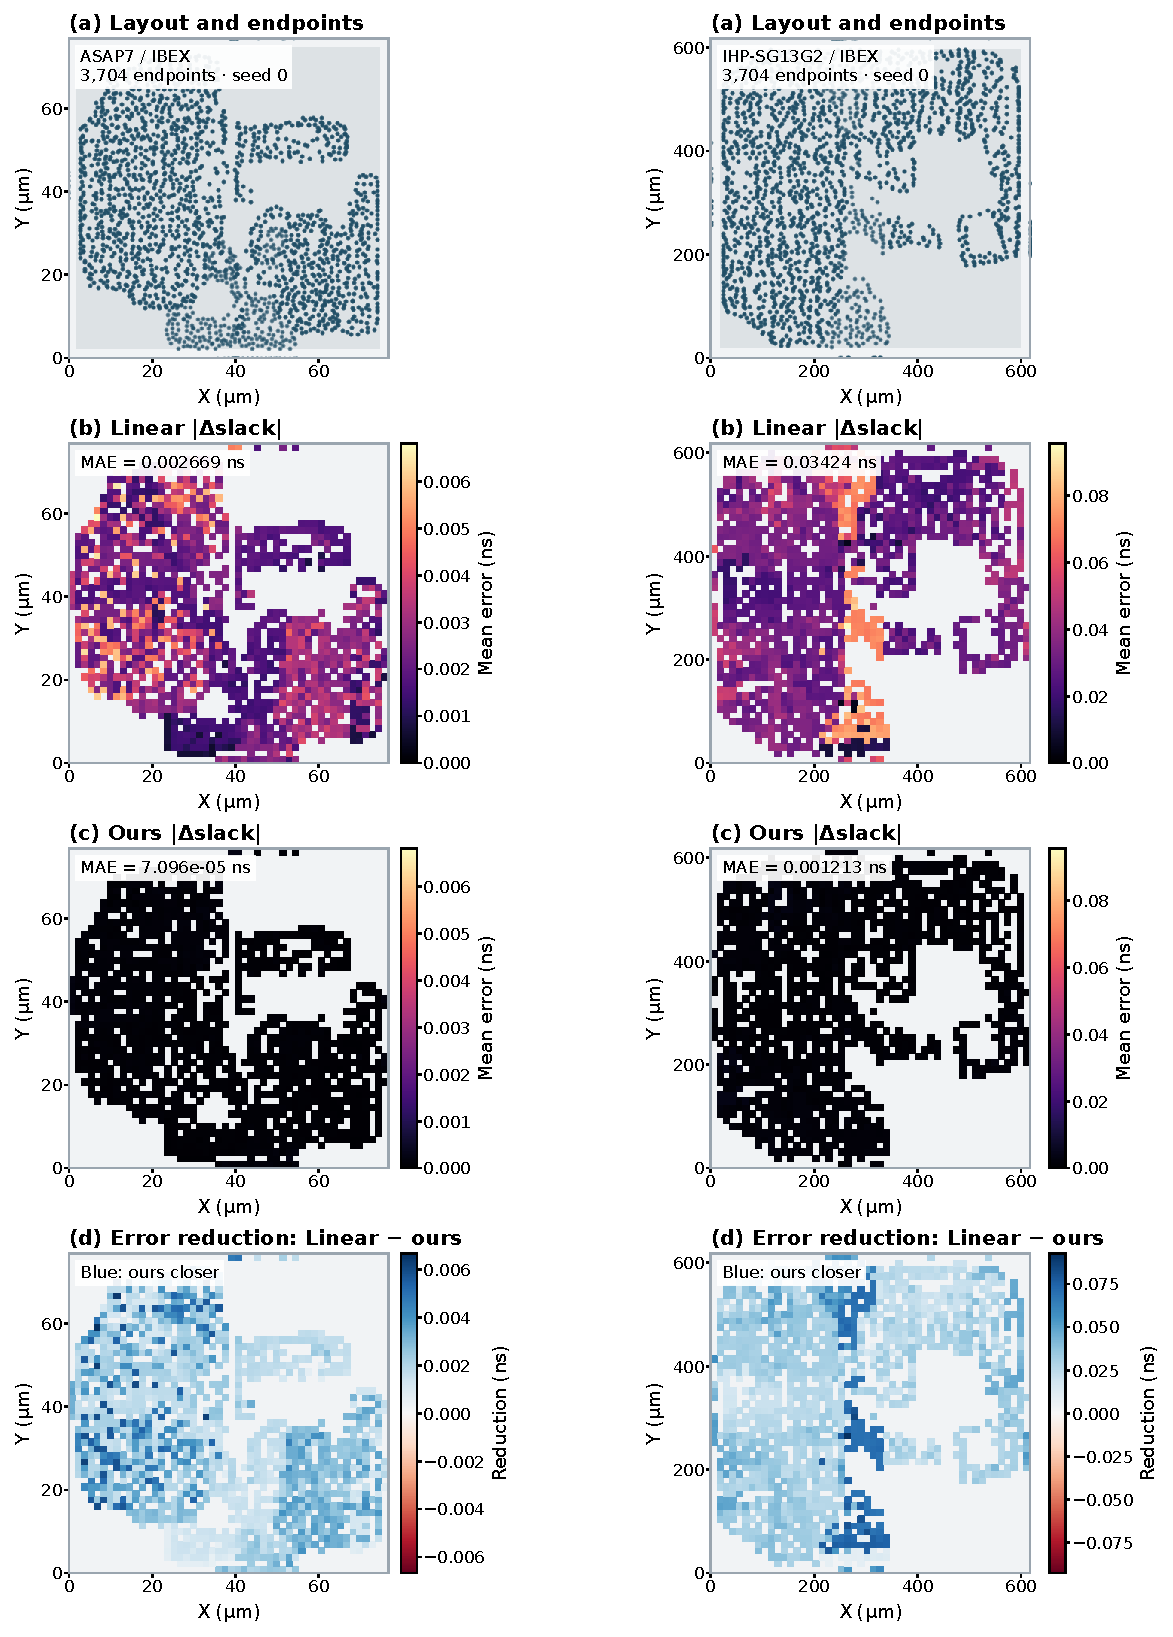
\includegraphics[width=\textwidth,height=0.79\textheight,keepaspectratio]{sta_visualization/additional_cases/figures/fig_sta_spatial_asap7_ihp.pdf}
\caption{\textbf{Spatial timing fidelity on ASAP7/IBEX (left) and IHP-SG13G2/IBEX (right).}
50\% block missingness, seed 0. Each column shows (a) placed cells and constrained
endpoints, (b) Linear absolute slack error, (c) ours and (d) error reduction
relative to Linear. Heatmaps average endpoint errors in $50\times50$ bins.
The two error maps share a scale within each column; reduction uses a symmetric
scale, with blue favoring ours. Gray bins are empty. Coordinates are in $\mu$m
and all errors in ns, including the converted ASAP7 exports.}
\label{fig:sta-spatial-asap7-ihp}
\end{figure}

\begin{figure}[p]
\centering
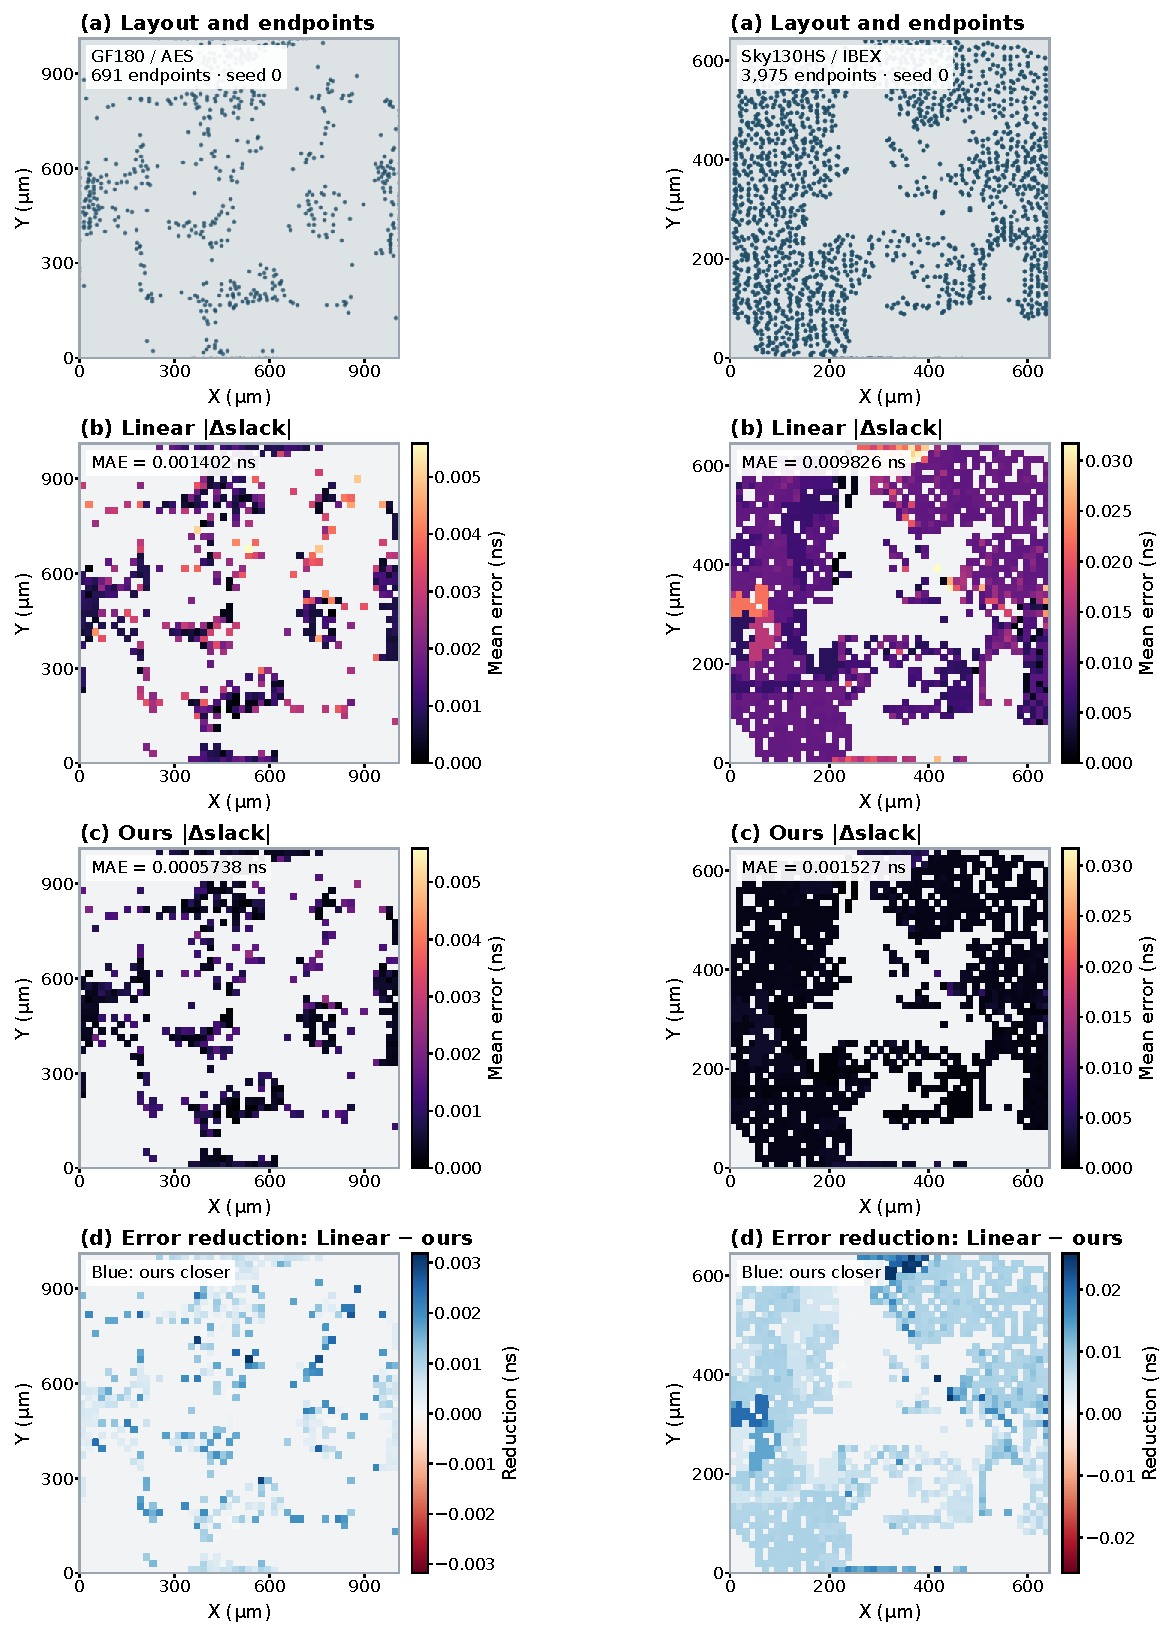
\includegraphics[width=\textwidth,height=0.79\textheight,keepaspectratio]{sta_visualization/additional_cases/figures/fig_sta_spatial_gf180_sky130.pdf}
\caption{\textbf{Spatial timing fidelity on GF180/AES (left) and Sky130HS/IBEX (right).}
50\% block missingness, seed 0. Rows show layout/endpoints, Linear error,
ours and error reduction, following Figure~\ref{fig:sta-spatial}.
The maps include all 691 and 3,975 constrained endpoints, respectively;
the sparse GF180/AES coverage leaves more empty bins.
Within each column, Linear and ours share the same error scale;
blue/red in the symmetric reduction map indicate improvement/degradation.
Physical extents and color limits are specific to each setting.}
\label{fig:sta-spatial-gf180-sky130}
\end{figure}

\section{Discussion and limitations}
\label{sec:limitations}
\label{app:limitations}

\paragraph{What the results say about the design.}
The matched-budget controls distinguish a strong learned residual
contribution from condition-dependent routing gains. The full hybrid model
has a larger advantage on the FEM reference than on public rules, while a
binary gate is better in two transfer conditions
(Appendix~\ref{app:matched-controls}). Public rules isolate the correction
because their anchor equals CMI; rank-two controls show that boundary handling
also contributes. Strong block-mask results and weaker random-mask transfer
suggest that the benefit depends on what the remaining support can already
resolve, rather than on a uniform advantage of learned prediction.

\paragraph{Where the evidence stops.}
Extrapolation is measured relative to the observations retained by each mask.
The scored query geometries come from characterized reference tables; the
experiments do not establish accuracy arbitrarily far beyond those tables or
outside the source training distribution.
The FEM reference is a two-dimensional idealization, and source-only transfer
covers two related material stacks. Public rules are extraction references,
not independently solved physical truth. The downstream audit covers four
open processes and two designs with fixed layouts and held-out rewritten
tables; it measures extraction/STA agreement, not foundry signoff accuracy.
Numerical interpolation remains cheaper, and gate failures show that a useful
branch need not receive an appropriate weight. The failed descriptor-key
variants further caution against treating richer routing inputs as a sufficient
solution. The appendix retains these failures, small boundary cohorts and
all missingness rates alongside the positive main results.

\end{document}
